% report_exp_short.tex -- short synthesis of report_exp.tex (Part II, experimental data), written for readers who want the results
% Build: cd docs/latex && pdflatex report_exp_short (three passes; no bibtex)
% Every number is taken from report_exp.tex (fit ranges and edge positions of the bump slices from its source table
% tables_exp/res_bump.txt). Readability rewrite of 16 Nov 2026: results only, no internal labels, a plain "Selection:" sentence in
% every caption, the PT3 definition of the analyst (16 Nov 2026); the previous version is kept in the backup folder of the
% integration step.
\documentclass[11pt,a4paper]{article}
\usepackage[T1]{fontenc}
\usepackage[utf8]{inputenc}
\usepackage{lmodern}
\usepackage[margin=2.0cm]{geometry}
\usepackage{amsmath}
\usepackage{graphicx}
\usepackage{booktabs}
\usepackage{tabularx}
\usepackage{longtable}
\usepackage{xcolor}
\usepackage{caption}
\usepackage{float}
\usepackage{microtype}
\usepackage{xspace}
\usepackage[colorlinks=true,linkcolor=blue!50!black,urlcolor=blue!50!black]{hyperref}

\captionsetup{font=small,labelfont=bf,margin=0.3cm}
\setlength{\parskip}{0.4em}
\setlength{\parindent}{0pt}
\setlength{\emergencystretch}{3em}
\renewcommand{\arraystretch}{1.15}
\newcolumntype{L}{>{\raggedright\arraybackslash}X}

\newcommand{\pip}{\ensuremath{\pi^{+}}\xspace}
\newcommand{\pim}{\ensuremath{\pi^{-}}\xspace}
\newcommand{\piz}{\ensuremath{\pi^{0}}\xspace}
\newcommand{\ee}{\ensuremath{e^{+}e^{-}}\xspace}
\newcommand{\pipi}{\ensuremath{\pi^{+}\pi^{-}}\xspace}
\newcommand{\ppee}{\ensuremath{\pi^{+}\pi^{-}e^{+}e^{-}}\xspace}
\newcommand{\Mfour}{\ensuremath{M(\pi^{+}\pi^{-}e^{+}e^{-})}\xspace}
\newcommand{\Mee}{\ensuremath{M(e^{+}e^{-})}\xspace}
\newcommand{\Mpipi}{\ensuremath{M(\pi^{+}\pi^{-})}\xspace}
\newcommand{\betanew}{\ensuremath{\beta_{\mathrm{new}}}\xspace}
\newcommand{\nbinv}{\ensuremath{\mathrm{nb}^{-1}}\xspace}
\newcommand{\GeVc}{\ensuremath{\mathrm{GeV}/c}\xspace}
\newcommand{\GeVcc}{\ensuremath{\mathrm{GeV}/c^{2}}\xspace}
\newcommand{\MeVcc}{\ensuremath{\mathrm{MeV}/c^{2}}\xspace}
\newcommand{\MMfour}{\ensuremath{\mathrm{MM}_4}\xspace}
\newcommand{\dzpi}{\ensuremath{\Delta z_\pi}\xspace}
\newcommand{\alab}{\ensuremath{\alpha_{\mathrm{lab}}}\xspace}
\newcommand{\vz}{\ensuremath{v_z}\xspace}
\newcommand{\fwin}{\ensuremath{f_{\mathrm{win}}}\xspace}
\newcommand{\feta}{\ensuremath{f_\eta}\xspace}
\newcommand{\Medge}{\ensuremath{M_{\mathrm{edge}}}\xspace}% the kinematic edge of the bump for the measured masses of a count
\newcommand{\keybox}[1]{\par\noindent\fcolorbox{blue!50!black}{blue!5}{\parbox{\dimexpr\linewidth-2\fboxsep-2\fboxrule\relax}{#1}}\par}
\newcommand{\inshort}[1]{\par\noindent\fcolorbox{blue!30}{blue!3}{\parbox{\dimexpr\linewidth-2\fboxsep-2\fboxrule\relax}{\textbf{In short:} #1}}\par}
% plain-words selection phrases, written out in full in every caption (the analyst's instruction of 15 Nov 2026: every caption
% states the exact cuts and their values); PT3 in the words of the analyst's definition (16 Nov 2026)
\newcommand{\selptthree}{PT3 trigger (at least two sectors with an inner-TOF hit in coincidence with TOF or RPC, and at least three
inner-TOF paddles hit; trigger bit 8192)\xspace}
\newcommand{\selpid}{particles identified by their START-free velocity \betanew (pions within $3\sigma$, leptons within $5\sigma$ of the
expected band; leptons with a RICH ring, pions without)\xspace}
\newcommand{\selcor}{energy-loss-corrected momenta for all four tracks (none exists for a \pim below $16^\circ$)\xspace}
\newcommand{\selall}{all stored \ppee combinations of each event\xspace}
\newcommand{\selbase}{\selptthree; an event vertex inside the target region, $\vz>-160$\,mm; \selpid; \selcor; \selall}
\newcommand{\selvtx}{both pion tracks used in the fit of the event vertex\xspace}
\newcommand{\seldz}{both pion tracks within 40\,mm of the event vertex along the beam ($\dzpi<40$\,mm)\xspace}
\newcommand{\selmm}{missing mass of \ppee below 2.85\,\GeVcc ($\MMfour<2.85$\,\GeVcc)\xspace}
\newcommand{\selpeaknom}{angle between the \pipi and the \ee momenta in the laboratory below $55^\circ$ ($\alab<55^\circ$) and $\Mpipi>0.30$\,\ensuremath{\mathrm{GeV}/c^{2}}\xspace}
\newcommand{\selbumpnom}{$\alab<40^\circ$ and $0.30<\Mpipi<0.41$\,\ensuremath{\mathrm{GeV}/c^{2}}\xspace}
\newcommand{\selcb}{CB $=2\sqrt{N_{++}N_{--}}$ from the like-sign counts ($\pipi e^+e^+$, $\pipi e^-e^-$) with the same cuts, in
10\,\MeVcc cells of \Mfour, no extra factor ($k=1$)\xspace}
\newcommand{\selfit}{a Gaussian fixed at 0.5439\,\GeVcc with width 5.4\,\MeVcc plus a second-order polynomial, fitted in
0.5225--0.6100\,\ensuremath{\mathrm{GeV}/c^{2}}\xspace}
% figure-heavy Results section: allow fuller float pages, and \floatbarrier (as placeins) keeps the result figures inside Section 1
\renewcommand{\topfraction}{0.9}\renewcommand{\bottomfraction}{0.6}\renewcommand{\textfraction}{0.07}\renewcommand{\floatpagefraction}{0.75}
\setcounter{topnumber}{3}\setcounter{bottomnumber}{2}\setcounter{totalnumber}{4}
\makeatletter
\newcommand{\floatbarrier}{\par\begingroup\let\@elt\relax\edef\@tempa{\@botlist\@deferlist\@dbldeferlist}\ifx\@tempa\@empty\else\clearpage\fi\endgroup}
\makeatother

\title{\Large $p + p \to \pi^{+}\pi^{-}e^{+}e^{-}$ Analysis Report\\[0.3em]
       \normalsize Short summary of Part II: the experimental data}
\author{W.~Przygoda}
\date{16 November 2026}

\begin{document}
\maketitle
\vspace{-1.6em}

\keybox{\textbf{\large Key results in plain words}\\[0.1em]
{\small HADES, p+p at 4.5\,GeV (beam time of February--March 2022), data only. A count is one stored \pip\pim$e^+e^-$ combination (an
event can give more than one); nothing is corrected for efficiency. Status: \emph{final} (re-derived independently with separate code),
\emph{measured} (from these data, not part of that re-derivation), \emph{provisional} (may still change), \emph{not determined} (needs the
simulation).
\begin{enumerate}\setlength{\itemsep}{1pt}\setlength{\topsep}{2pt}
\item \textbf{The $\eta$ peak is clearly seen} (Fig.~\ref{fig:fits}): content $S=4364\pm310\,(\mathrm{stat})\pm477\,(\mathrm{model})$ counts, i.e.\
      $0.73\pm0.05\pm0.08$ visible counts per nb$^{-1}$, with the recommended selection (base cuts, Section~\ref{sec:results}, plus
      both pion tracks within 40\,mm of the event vertex along the beam and missing mass below 2.85\,\GeVcc; chosen on the simulation). In
      the six candidate $\eta$-peak selections of the full report $S$ is 12.7--14.3 times its statistical and 7.6--8.6 times its total
      error; these ratios compare selections and are not significances. \emph{Final.}
\item \textbf{The bump} ($\eta\to\pi^+\pi^-\pi^0$, $\pi^0\to e^+e^-\gamma$, photon lost) \textbf{is seen through its kinematic edge}
      (Fig.~\ref{fig:bump}), exactly where expected: with the base cuts the edge steps of four \Mpipi slices sum to
      $E=1199\pm71\,(\mathrm{stat})\pm287\,(\mathrm{model})$ counts per 2.5\,\MeVcc, \emph{final}, a visibility measure, not a yield.
      \textbf{In the distance to the edge}, $u$, all edges fall on $u=0$: with both pion tracks also in the vertex fit, \textbf{one sharp
      step of $1308\pm62$ counts per 2.5\,\MeVcc} (21$\sigma$; Fig.~\ref{fig:edgeu}; \emph{measured}). In $u$ the $e^-e^-$ counts step by
      $73.5\pm15.7$ counts per 2.5\,\MeVcc (4.7$\sigma$): pairs from the two photons of the \piz, which the CB subtracts as it should. The
      bump yield is \emph{not determined} here (Part~III, data with simulation, measures it).
\item \textbf{The combinatorial background (CB, $e^+$ and $e^-$ from different sources) is small, and the $\eta$ results hardly depend on it}
      (Figs.~\ref{fig:res-cb} and~\ref{fig:res-cbnull}): 7--10\,\% of the counts in the peak window (5.5\,\% for the data-tuned selection,
      1.9\,\% in the X17 search band); $\pm3$\,\% moves $S$ by $<0.1$\,\%, a 38--45\,\% larger CB by $\le1$\,\% (up to 2.3\,\% with
      only the best-ranked combination of each event and in the X17 search band). \emph{Final}; its absolute scale is \emph{not
      determined} (not checkable with data alone).
\item \textbf{The selection chosen on the simulation is as good as the best one tuned on the data} (Fig.~\ref{fig:res-selection}): it raises
      the precision $S/\mathrm{stat}$ from 12.7 to 14.1, the same gain as the best blind choice on the data ($+1.35$ against $+1.36$).
      \emph{Provisional.}
\item \textbf{The event-vertex cut keeps $99.4\pm2.1$\,\% of the $\eta$} (Fig.~\ref{fig:res-vertex}; \emph{measured}); the 32\,\% of the
      counts it removes are mostly not p+p collisions in the hydrogen (probably beam halo on material in front of the cell) and hold no
      measurable $\eta$.
\item \textbf{Normalisation} (Figs.~\ref{fig:res-norm} and~\ref{fig:res-walls}): luminosity $L=6079.2\,\mathrm{nb}^{-1}\pm6.9$\,\%; three
      uncorrected one-sided effects (trigger live fraction, a trigger loss in one sector on the first days, events lost in the track
      reconstruction) could make the yields up to about 11\,\% too low, and rate steps between beam periods add $\pm5$\,\% (they follow
      the beam-halo level: an indication). \textbf{The target walls} (127 empty-target runs) give 13--15\,\% of the counts after CB
      subtraction in 0.40--0.70\,\GeVcc (both pions in the vertex fit; 19\,\% with the base cuts alone, raw) but only $3^{+4}_{-3}$\,\% of
      the $\eta$ signal (\emph{measured}, not subtracted). \emph{Provisional} (the bookkeeping of $L$ is final).
\item \textbf{Inside the peak, close pairs dominate} (Fig.~\ref{fig:res-mee}): about 40\,\% of the peak is an excess of \ee pairs of
      5--20\,\MeVcc, which would fit $\eta\to\pi^+\pi^-\gamma$ with the photon converted in the material; 0.23 of the peak lies above
      20\,\MeVcc. \emph{Provisional}: the data alone do not prove it.
\item \textbf{Nothing unusual where an X17 boson would appear} (\Mee 15.5--24.5\,\MeVcc, Fig.~\ref{fig:res-x17}): $481\pm99$ $\eta$ counts
      where $522\pm111$ are expected from the neighbouring \ee masses; a limit needs the simulated efficiency (\emph{not determined}
      here; Part~III derives it).
\end{enumerate}
Evidence and meaning: Section~\ref{sec:results}; open points: Section~\ref{sec:open}; how each number was obtained: the full report
\texttt{report\_exp.pdf}, whose Appendix~B lists the analysis decisions behind these results.}}

%======================================================================
\section{Results}
\label{sec:results}
%======================================================================
\inshort{The $\eta$ meson is seen in two ways in the data alone: as a peak at its mass and as the kinematic edge of the bump below it.
Both are robust against the combinatorial background, the selection and the event-vertex cut; the visible yields carry the luminosity
uncertainty, three one-sided effects and a period normalisation, and the target walls contribute almost none of the $\eta$.}

\textbf{The data.} The HADES p+p beam time of February--March 2022 (days 034--067 of 2022), at a beam kinetic energy of 4.5\,GeV (4530\,MeV
in the kinematics): 29 days of data, reconstructed without the time of the START detector (the start-time detector in front of the target).
Two $\eta$ signals are expected in the mass of the four particles, \Mfour: the \emph{peak} at the $\eta$ mass ($\eta\to\ppee$, and
$\eta\to\pipi\gamma$ with the photon converted into an \ee pair in the detector material) and the \emph{bump} below it ($\eta\to\pipi\piz$,
$\piz\to\ee\gamma$, with the photon lost). Three rules hold for every number: a count is one stored \ppee combination of four tracks,
and an event can give more than one count; nothing is corrected for acceptance or efficiency; a yield per luminosity is a \emph{visible}
yield in visible counts per \nbinv, not a cross section.

\textbf{The trigger.} All counts come from PT3, the main reaction trigger of this beam time: at least two of the six sectors with a hit
in the inner TOF wall (iTOF) in coincidence with a hit in the outer TOF wall or in the RPC of the same sector, and at least three iTOF
paddles hit. PT2, the minimum-bias trigger (at least one such sector), is downscaled by 64 and is the trigger from which the luminosity
is made. Only the bit of the trigger signal that arrives first is written: PT3 events carry bit 8192, while the downscaled PT2 events
and the events with both PT2 and PT3 carry 4096. The events with bit 8192 therefore hold 63/64 of all PT3 events, and every yield is
multiplied by 64/63. (Definition: P.~Tlusty, ``LVL1 trigger in Feb22 p+p 4.5\,GeV'', HADES internal presentation, 13 December 2024,
with the definition slide of I.~Ciepa{\l}.)

\textbf{Base cuts}, part of every selection of this report: \selbase. They keep 4\,423\,338 \ee, 85\,921 $e^+e^+$ and 267\,362
$e^-e^-$ counts. Table~\ref{tab:sel} lists the selections built on them.

\textbf{Background and peak fit.} The combinatorial background is \selcb, interpolated to 2.5\,\MeVcc. The $\eta$-peak content $S$ comes
from a fit of $N-\mathrm{CB}$ with \selfit (``the peak fit''); $S$ is the content of the whole Gaussian. Mass windows on the data scale:
peak window 0.53364--0.55416\,\GeVcc, bump window 0.4550--0.5225\,\GeVcc.

\begin{table}[htb]
\centering
\caption{\textbf{Selections used in this report.} Each one consists of the base cuts (\selbase) plus the cuts in the second column. The
names in the first column are plain descriptions used in the text.}
\label{tab:sel}
\footnotesize
\begin{tabularx}{\textwidth}{@{}>{\raggedright\arraybackslash}p{3.0cm} >{\raggedright\arraybackslash}p{4.4cm} L@{}}
\toprule
Selection & Cuts on top of the base cuts & Property \\
\midrule
recommended $\eta$-peak selection & \seldz; \selmm & chosen on the simulation alone (Part~I, the simulation report), so free of a
   data-optimisation bias; the data keep the same share of the $\eta$ as the simulation ($\dzpi$ cut: $0.961\pm0.034$ / 0.963; \MMfour cut:
   $0.972\pm0.023$ / 0.967; the simulation was made at a beam energy of 4500\,MeV, the data kinematics use 4530\,MeV); the missing-mass
   cut can make a small fake peak content from a smooth spectrum, $+48\pm27$ or $+83\pm26$ counts depending on how the smooth spectrum
   is modelled (one-sided, $\le1.9$\,\%) \\
bump edge selection & none & used for the edge step $E$; no cut touches the bump edge \\
step in the distance to the edge & \selvtx; $0.30\le\Mpipi<0.40$\,\GeVcc; $\Mee<135$\,\MeVcc & used for the step $h_u$ (Section~\ref{sec:bump}) \\
X17 search & \selvtx; $15.5\le\Mee<24.5$\,\MeVcc (the X17 search band) & cuts chosen on the simulation; Part~III searches in the simulated
   \Mfour window moved to the data mass scale ($\times0.5439/0.5460$), $0.5312\le\Mfour<0.5566$\,\GeVcc: $N=6395\pm81$, CB $=124\pm16$;
   the data-only look of this report (Fig.~\ref{fig:res-x17}) uses the narrower peak window 0.53364--0.55416\,\GeVcc \\
pion-distance cut alone & \seldz & cross-check, also chosen on the simulation; against the recommended selection it tests the missing-mass cut \\
data-tuned peak selection & \selpeaknom; \selvtx & cross-check, tuned on these data; carries an optimisation bias of about 0.4 in $S/\mathrm{stat}$ \\
data-tuned bump selection & \selbumpnom; \selvtx & cross-check, tuned on these data \\
variants & only the best-ranked combination of each event; or \ee opening angle above $2^\circ$ & cross-checks; the opening-angle cut is never used as a selection \\
\bottomrule
\end{tabularx}
\end{table}

%----------------------------------------------------------------------
\subsection{The \texorpdfstring{$\eta$}{eta} peak}
\label{sec:peak}
\textbf{The $\eta$ peak is clearly seen.} With the recommended selection $S=4364\pm310\,(\mathrm{stat})\pm477\,(\mathrm{model})$ counts,
a visible yield $Y=S\times\frac{64}{63}/L=0.729\pm0.052\pm0.080$ visible counts per \nbinv (Fig.~\ref{fig:fits}). In the six candidate
$\eta$-peak selections of the full report (the base cuts alone, the pion-distance cut alone, the recommended and the data-tuned selection
shown here, and two further cut sets) $S$ is 12.7--14.3 times its statistical error and 7.6--8.6 times its total error; these ratios
compare selections and are not significances. The selections give 3949--4671 counts because their cuts keep different shares of the
$\eta$; only the simulated efficiencies make them comparable. The model uncertainty is the rms of $S$ over the variations of the fit
(polynomial order, fit range starting at 0.5225\,\GeVcc or above, Gaussian width) that pass a $\chi^2$ probability above 0.05: 9--11\,\% of
$S$, comparable to the statistical error (7--8\,\%); the width of the fixed Gaussian ($\pm0.5$\,\MeVcc) is its largest single source.
Independent halves of the data confirm the statistical errors. The peak sits at $0.9927\pm0.0009$ of the $\eta$ mass. \emph{Meaning:} the
$\eta$ signal in \ppee is established, as a raw count. \emph{Status:} final.

\begin{figure}[tbp]
\centering
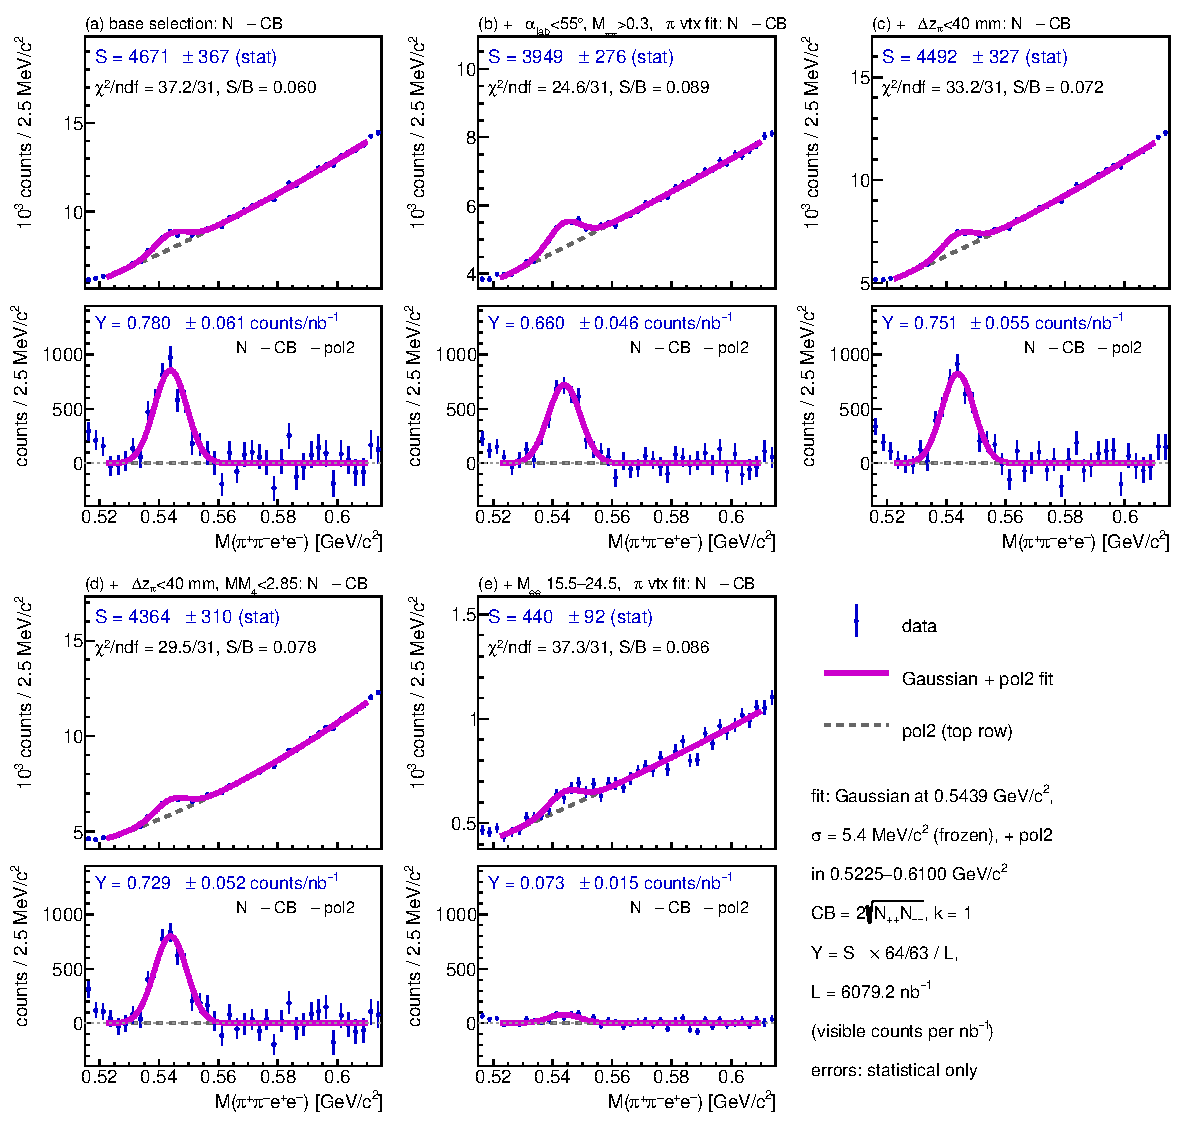
\includegraphics[width=0.96\textwidth]{figs_exp/res_peak_fits_cnt_short.pdf}
\caption{\textbf{What it shows: the $\eta$ peak stands out in every candidate selection; panel (d) is the recommended selection.}
Top of each panel: $N-\mathrm{CB}$ against \Mfour with the peak fit (magenta) and its polynomial alone (grey dashed); bottom: $N-\mathrm{CB}$
minus the polynomial, equal y ranges. Printed: $S$ with its statistical error, $\chi^2/\mathrm{ndf}$, $S/B$ (the part of $S$ in the peak
window over the polynomial + CB there) and $Y=S\times64/63/L$ with $L=6079.2$\,\nbinv. Statistical errors only (model uncertainties in
Table~\ref{tab:main}).
\emph{Selection:} data; \selbase; on top of that (a) nothing more; (b) \selpeaknom, and \selvtx; (c) \seldz; (d) \seldz and \selmm (the
recommended selection); (e) \selvtx and $15.5\le\Mee<24.5$\,\MeVcc (the X17 search band, no \Mfour window). \selcb. Peak fit: \selfit.
\emph{Words inside the figure:} ``base selection'' $=$ the base cuts; ``$\pi$ vtx fit'' $=$ \selvtx; $M_{\pi\pi}=\Mpipi$, $M_{ee}=\Mee$
(in \MeVcc), $\mathrm{MM}_4=$ missing mass; pol2 $=$ second-order polynomial; ``frozen'' $=$ fixed. Counts per 2.5\,\MeVcc, not
normalised to luminosity except $Y$.}
\label{fig:fits}
\end{figure}

%----------------------------------------------------------------------
\subsection{The bump}
\label{sec:bump}
\textbf{The bump is seen through its kinematic edge, exactly where expected} (Fig.~\ref{fig:bump}). The bump has no peak; its visible sign
is a drop of the spectrum at the largest \Mfour that $\eta\to\pipi\piz$ with a lost photon can reach. With the base cuts alone, the height
of this step summed over four \Mpipi slices is $E=1199\pm71\,(\mathrm{stat})\pm287\,(\mathrm{model})$ counts per 2.5\,\MeVcc; a bootstrap
of the data confirms the statistical error. Left free, the edge lies at $0.9927\pm0.0013$ of the kinematic limit, the same mass scale as
the $\eta$ peak. Control slices above the kinematic limit show no step. \emph{Meaning:} the $\eta\to\pipi\piz$ decays are seen where the
kinematics puts them. $E$ measures how visible the edge is; it is \emph{not a yield}, and the bump yield is not determined without the
simulation. \emph{Status:} final.

\textbf{In the distance to its edge, the bump is one sharp step} (Fig.~\ref{fig:edgeu}). Every count has its own edge,
$\Medge(\Mpipi,\Mee)$ (a heavier \ee pair leaves less energy to the lost photon); in the distance $u=\Mfour-\Medge$ all edges fall on $u=0$,
which needs no simulation. This measurement uses the base cuts with both pion tracks in the vertex fit, $0.30\le\Mpipi<0.40$\,\GeVcc and
$\Mee<135$\,\MeVcc (Table~\ref{tab:sel}). One fit of the data (polynomial + step) gives $h_u=1308\pm62$ counts per 2.5\,\MeVcc, 21$\sigma$
($\chi^2/\mathrm{ndf}=40.2/32$); with its width free the step is $6.3\pm0.7$\,\MeVcc wide, as expected from the mass resolution (the
simulated resolution at the edge is 6.7\,\MeVcc, the $\eta$ peak has 5.4\,\MeVcc), and $h_u=1271\pm85$. A control region above the
kinematic limit shows none. The $\eta$ peak enters the fit range above $u\approx+15$\,\MeVcc: a peak term built from the data gives
$1217\pm66$, the simulated peak shape (Part~III) $1305\pm62$, so the height is fixed to about 7\,\%. Of the 88 counts between the two,
about 50 come from the low-mass tail of the simulated peak (radiation of the leptons in the material) and about 40 from where the data put
the peak counts (1.0\,\MeVcc further from their edges than in the simulation, not understood). The data cannot measure the size of the
tail ($t=0.3\pm1.0$ times the simulated one); in Part~III it gives a $\pm3.4$\,\% uncertainty of the bump measurement. Like $E$, $h_u$ is
not a yield; Part~III turns it into its bump measurement: the data hold 0.426 times the bump predicted by SMASH, the transport-model
event generator of the simulation (with its $\eta$ production cross section and the PDG branching ratios). \emph{Status:} measured.

\textbf{The $e^-e^-$ like-sign counts also step at the edge in $u$, and the reason is known} (Figs.~\ref{fig:edgeu}c and~\ref{fig:eesteps}):
$73.5\pm15.7$ counts per 2.5\,\MeVcc (4.7$\sigma$), against $2.1\pm6.5$ for $e^+e^+$. None was expected from leptons of unrelated sources.
They are pairs of leptons from the \emph{two different photons} of the \piz in $\eta\to\pipi\piz$ (a Dalitz $e^-$ and a conversion
$e^-$, or two conversion $e^-$): kinematics gives them exactly the edge of the bump, and near it they are heavy. In the data the
$e^-e^-$ step lies at $\Mee\ge90$\,\MeVcc ($57.0\pm9.1$, 6.3$\sigma$) and not below 50\,\MeVcc ($3.6\pm8.9$), where the bump is. At
$\Mee\ge90$\,\MeVcc the $e^+e^+$ counts step too, but less ($7.3\pm4.3$): soft $e^+$ are accepted less often than soft $e^-$, and a photon
can also give a Compton or knock-on electron, which is always negative. It is not a wrong charge sign of the Dalitz $e^+$ (that would put
the step at small \Mee). Each such decay also gives \ee cross pairs, and the unlike-sign counts carry them: at $\Mee\ge90$\,\MeVcc $N$
steps by $52.6\pm10.9$ and the CB by $35.8\pm8.6$. \emph{Meaning:} the CB subtracts these pairs as it should (39 counts, 3\,\% of $h_u$);
the $\eta$ peak and the X17 search band are not affected. \emph{Status:} measured.

\begin{figure}[tbp]
\centering
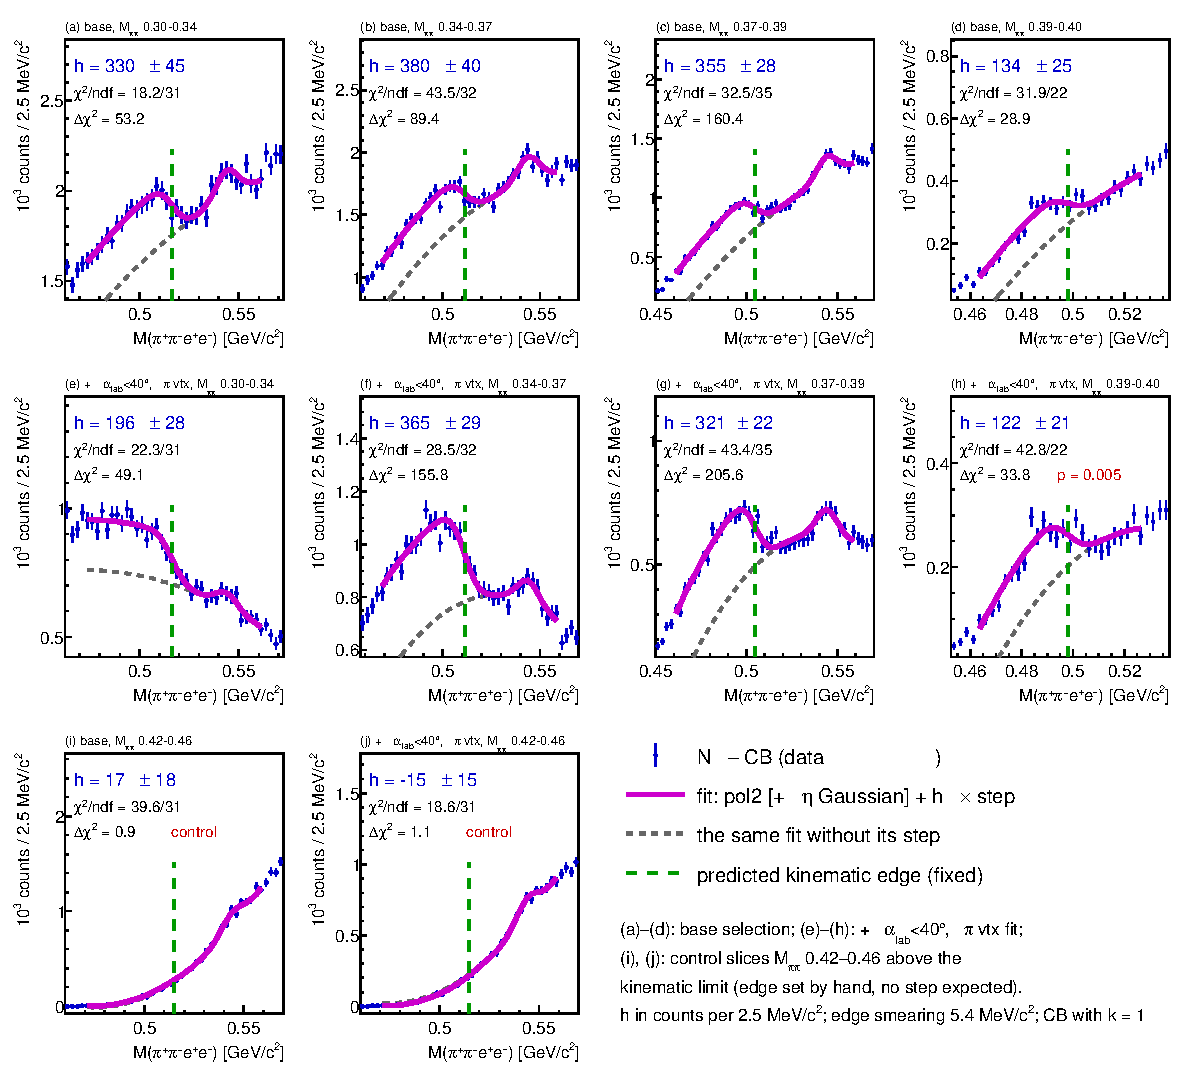
\includegraphics[width=\textwidth]{figs_exp/res_bump_slices_cnt_short.pdf}
\caption{\textbf{What it shows: the bump appears as a step at the predicted kinematic edge, in every \Mpipi slice, and not in the control
slices above the kinematic limit.} Blue: $N-\mathrm{CB}$ against \Mfour; magenta: fit of a second-order polynomial (plus the $\eta$
Gaussian where the peak is in range) and a step of height $h$ at the predicted kinematic edge (green dashed, fixed; step smeared by
5.4\,\MeVcc); grey dashed: the same fit without the step. Predicted edges and fit ranges: (a, e) 0.5166, fitted in 0.4725--0.5625; (b, f)
0.5113, in 0.4675--0.5600; (c, g) 0.5048, in 0.4600--0.5600; (d, h) 0.4981, in 0.4625--0.5275; (i, j) 0.5150 (set by hand), in
0.4700--0.5600\,\GeVcc. Printed: $h$ (counts per 2.5\,\MeVcc), $\chi^2/\mathrm{ndf}$ and the $\chi^2$ gain of the step, $\Delta\chi^2$. $E$
is the sum of $h$ over (a)--(d): $330+380+355+134=1199$. The fit of (h) has a $\chi^2$ probability of only 0.005.
\emph{Selection:} data; \selbase; all \Mee; \Mpipi slices (a, e) 0.30--0.34, (b, f) 0.34--0.37, (c, g) 0.37--0.39, (d, h)
0.39--0.40\,\GeVcc, and (i, j) the control slice 0.42--0.46\,\GeVcc above the kinematic limit (no step expected); (a)--(d) and (i):
nothing more; (e)--(h): \selbumpnom, and \selvtx; (j): $\alab<40^\circ$ and \selvtx. \selcb.
\emph{Words inside the figure:} ``base'' $=$ the base cuts; ``$\pi$ vtx'' $=$ \selvtx; $M_{\pi\pi}=\Mpipi$; pol2 $=$ second-order
polynomial. Counts per 2.5\,\MeVcc, not normalised to luminosity.}
\label{fig:bump}
\end{figure}

\begin{figure}[tbp]
\centering
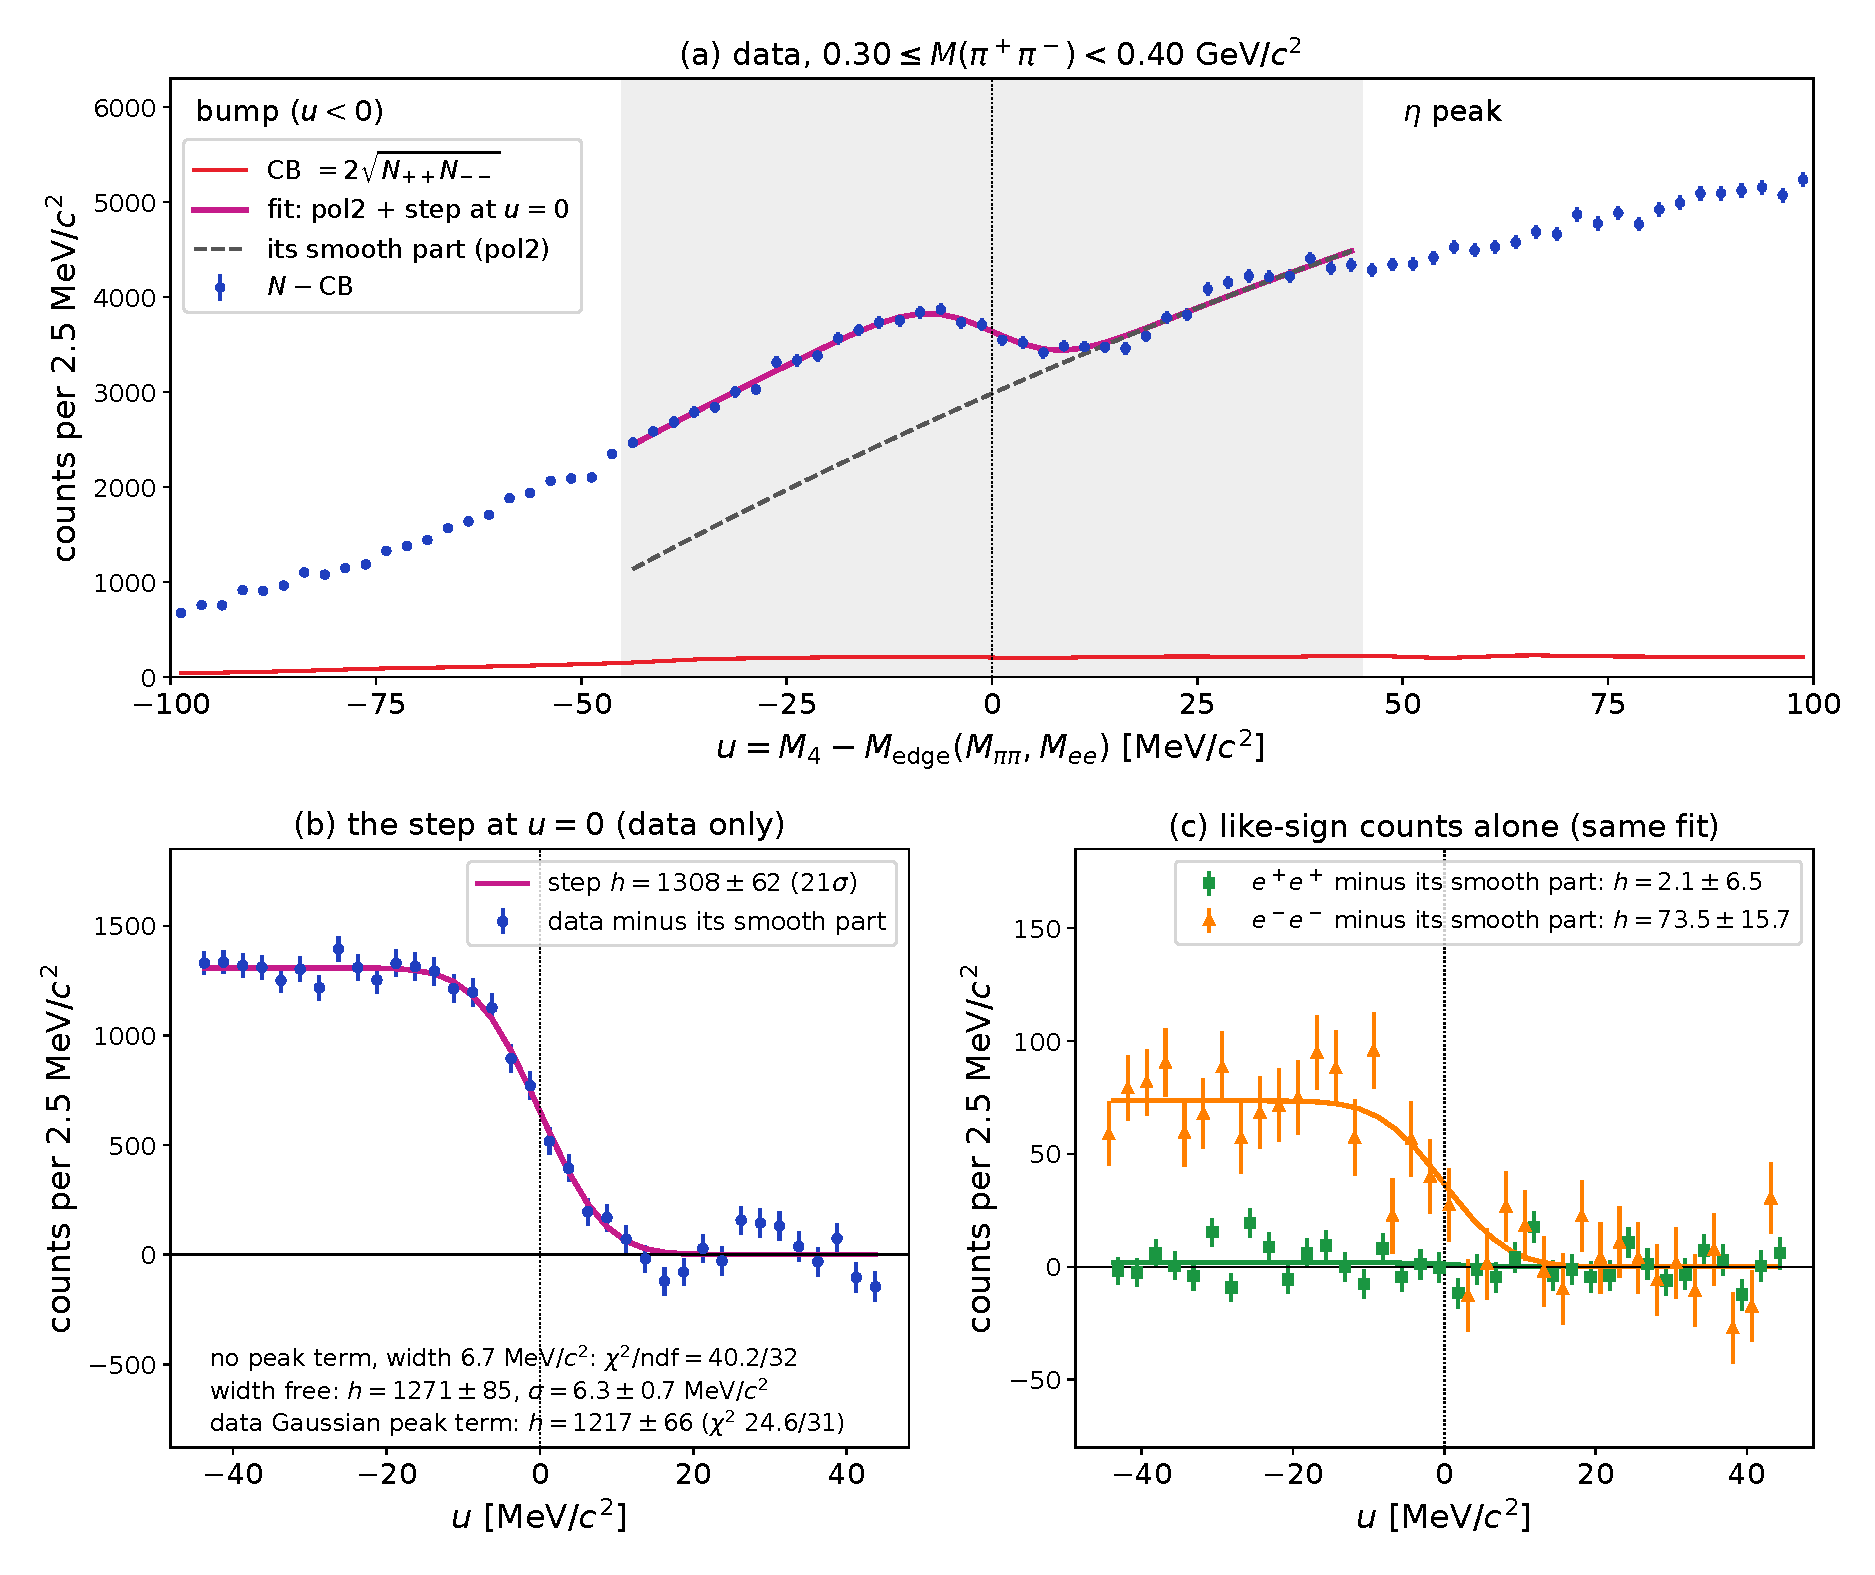
\includegraphics[width=0.86\textwidth]{figs_exp/p12w_edgeu_data_step_cnt.pdf}
\caption{\textbf{What it shows: in the distance to its edge, $u$, the bump is one sharp step at $u=0$; the like-sign counts step only a
little, almost all of it in $e^-e^-$ (pairs from the two \piz photons, at large \Mee).}
$u=\Mfour-\Medge(\Mpipi,\Mee)$, with \Medge the kinematic edge of $\eta\to\pipi\piz$, $\piz\to\ee\gamma$ (photon lost) for the measured
masses of the combination. (a, top) $N-\mathrm{CB}$ (blue), CB (red), fit with a second-order polynomial and a step at $u=0$ smeared with
6.7\,\MeVcc (the simulated resolution at the edge; the $\eta$ peak has 5.4\,\MeVcc) (magenta) on $-45\le u<+45$\,\MeVcc (grey band) and
its smooth part (dashed); the bump lies at $u<0$, the $\eta$ peak enters above $u\approx+15$\,\MeVcc. (b, bottom left) Data minus the
smooth part: the step, $h_u=1308\pm62$ counts (21$\sigma$); with the width free $1271\pm85$, with a Gaussian peak term from the data
$1217\pm66$. (c, bottom right) The like-sign counts alone with the same fit: $e^+e^+$ $2.1\pm6.5$, $e^-e^-$ $73.5\pm15.7$ counts
(4.7$\sigma$; Fig.~\ref{fig:eesteps}).
\emph{Selection:} data; \selbase; \selvtx; $0.30\le\Mpipi<0.40$\,\GeVcc; $\Mee<135$\,\MeVcc (the \piz mass; above it the edge is not
defined); CB $=2\sqrt{N_{++}N_{--}}$ from the like-sign counts with the same cuts, in 10\,\MeVcc cells of $u$, separately in the \Mpipi
slices 0.30--0.34, 0.34--0.37, 0.37--0.39 and 0.39--0.40\,\GeVcc, $k=1$.
\emph{Words inside the figure:} $M_4=\Mfour$, $M_{\pi\pi}=\Mpipi$, $M_{ee}=\Mee$; pol2 $=$ second-order polynomial. Counts per
2.5\,\MeVcc, not normalised to luminosity.}
\label{fig:edgeu}
\end{figure}

\begin{figure}[tbp]
\centering
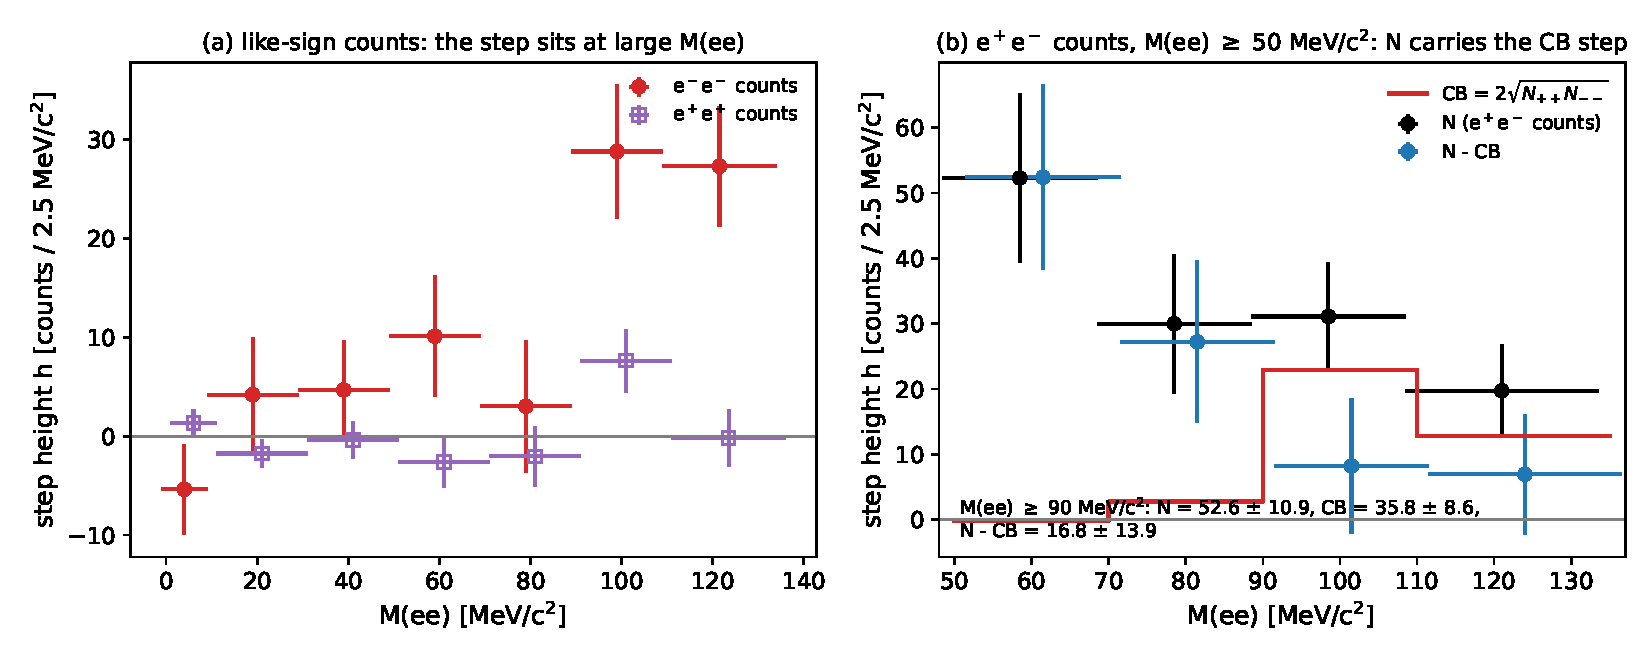
\includegraphics[width=\textwidth]{figs_exp/eestep_bands_data_cnt.pdf}
\caption{\textbf{What it shows: the like-sign step at the bump edge sits at large \Mee, where lepton pairs from the two \piz photons lie, and
there the unlike-sign counts carry the matching step, which the CB subtracts.} Step height at $u=0$ (counts per 2.5\,\MeVcc) of the fit of
Fig.~\ref{fig:edgeu}, per \Mee band 0--10, 10--30, 30--50, 50--70, 70--90, 90--110 and 110--135\,\MeVcc. (a) Like-sign counts: $e^-e^-$
(red), $e^+e^+$ (violet). (b) Unlike-sign counts at $\Mee\ge50$\,\MeVcc: $N$ (black), the CB of each band from its own like-sign counts (red
line), $N-\mathrm{CB}$ (blue).
\emph{Selection:} data; \selbase; \selvtx; $0.30\le\Mpipi<0.40$\,\GeVcc; the step fit of Fig.~\ref{fig:edgeu} done separately in each
\Mee band; CB of each band from the like-sign counts of that band, $k=1$.
\emph{Words inside the figure:} M(ee) $=\Mee$. Counts, not normalised to luminosity.}
\label{fig:eesteps}
\end{figure}

%----------------------------------------------------------------------
\subsection{The combinatorial background}
\label{sec:cb}
\textbf{The CB is small, and the $\eta$ results hardly depend on it} (Figs.~\ref{fig:res-cb} and~\ref{fig:res-cbnull}). In the peak window
CB$/N$ is 0.103 (base cuts alone), 0.076 (pion-distance cut), 0.072 (recommended selection), 0.055 (data-tuned peak selection) and 0.019
(X17 search band); the vertex cuts (the target-region cut and the two pion-vertex conditions) remove the CB two to three times more
strongly than the \ee counts. Most of the background under the peaks is physical (true \ee pairs with pions), which the polynomial of the
fits describes. A CB change of $\pm3$\,\% moves $S$ by at most 0.07\,\% and $E$ by at most 0.1\,\%; event mixing gives a CB factor of
1.01--1.04 in the signal regions (1.03--1.08 for the data-tuned bump selection and its variants), and applying it changes $S$ and $E$ by less
than 0.7\,\%; CB cells of 2.5, 5 or 20\,\MeVcc move $S$ by $-1.6$\dots$+2.1$\,\%, mostly the statistical noise of the CB estimate. Even the
plain sum $N_{++}+N_{--}$, a CB larger by 38--45\,\%, changes $S$ by at most 1\,\% (best-ranked combination only and the X17 search band:
up to 2.3\,\%), $E$ by at most 3\,\% and the $N-\mathrm{CB}$ counts of the bump window by up to $-7$\,\%. The like-sign counts show no
$\eta$ peak (the peak fit on $N_{++}+N_{--}$ gives $-56\pm132$ against $4671\pm367$ in $N-\mathrm{CB}$; moved to 46 positions it gives
pulls with rms 0.83--1.12) and no bump edge in \Mfour ($0.5\pm25.6$). \emph{Limits:} the absolute normalisation of the CB is not known.
$N_{--}/N_{++}$ is 5.4 in the peak window and 6.2 in the bump window, against 1.17 expected for independent leptons (single $e^-/e^+$:
1.08): correlated $e^-e^-$ sources exist, which event mixing cannot see, so CB$/N$ and the window counts carry an unknown scale ($k=1$ is
a convention). With only the best-ranked combination of each event, the formula is expected to give a CB 14--17\,\% too high (this does
not concern the results, which use all combinations). \emph{Status:} shares, null tests and sensitivities final; $k=1$ provisional; the CB
normalisation not determined.

\begin{figure}[tbp]
\centering
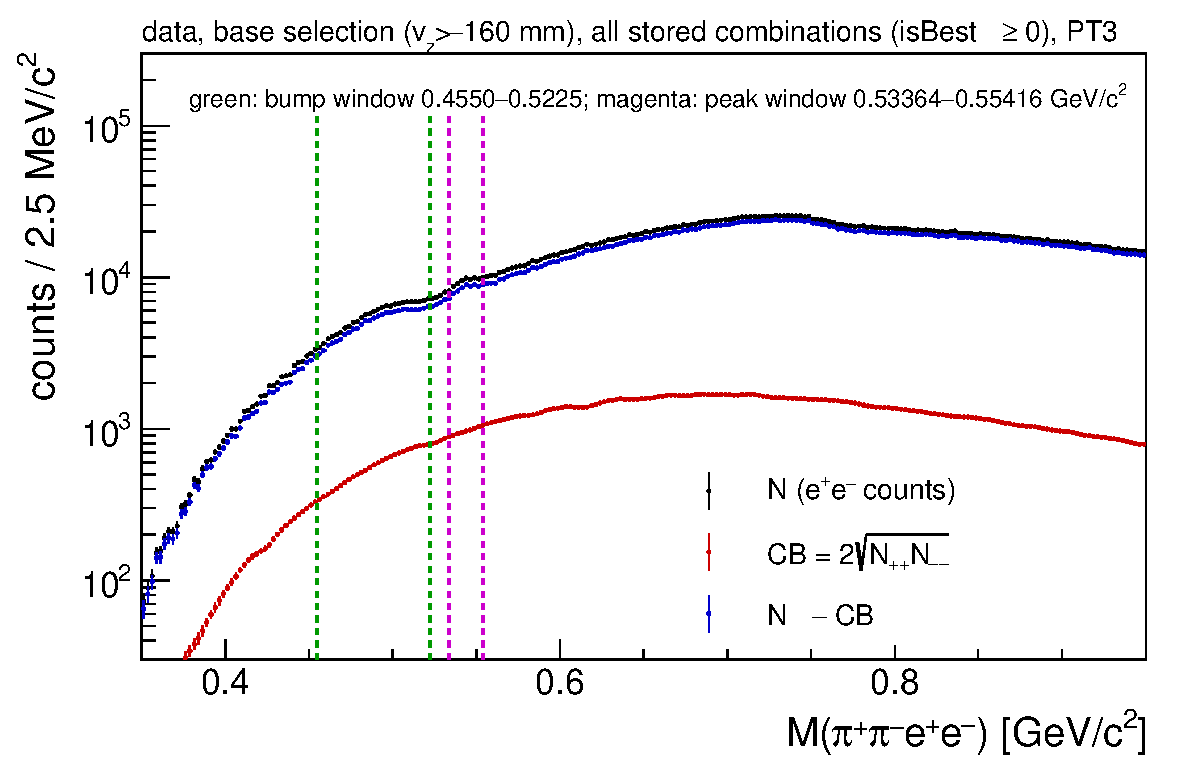
\includegraphics[width=0.62\textwidth]{figs_exp/res_peak_overview_cnt_plain.pdf}\\[0.2em]
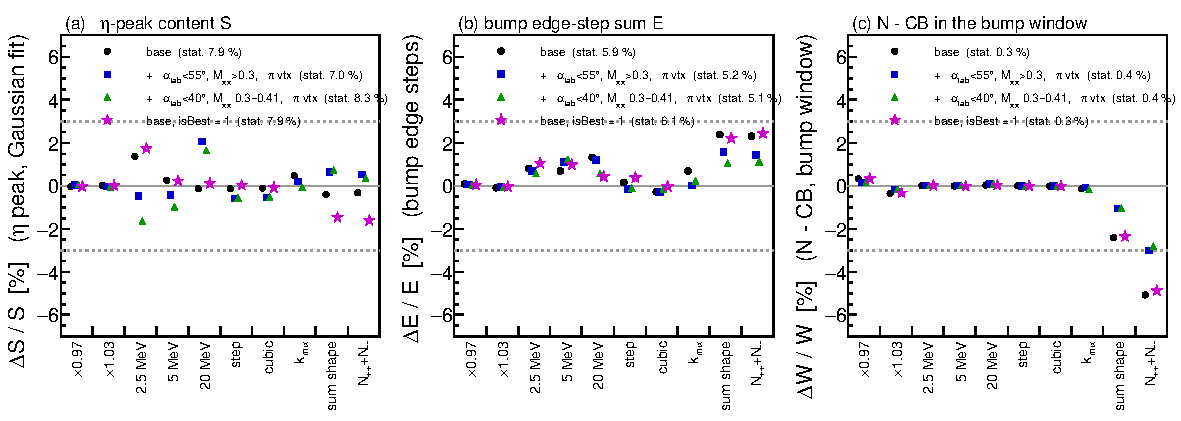
\includegraphics[width=\textwidth]{figs_exp/cb_sensitivity_plain.pdf}
\caption{\textbf{What it shows: the CB is small, and changing it barely moves the $\eta$ results.}
Top: \Mfour, black $N$, red CB, blue $N-\mathrm{CB}$; 2.5\,\MeVcc bins, log scale; green lines: bump window 0.4550--0.5225\,\GeVcc;
magenta lines: peak window 0.53364--0.55416\,\GeVcc, where CB$/N$ is 0.103 (0.072 for the recommended selection). Bottom: change in per
cent, when the CB estimate is changed, of (a) the $\eta$-peak content $S$, (b) the bump edge-step sum $E$ and (c) $N-\mathrm{CB}$ in the
bump window (legends: statistical error of each quantity). Variants along the x axis: CB $\times0.97$ and $\times1.03$ (at most 0.07\,\% on
$S$, 0.1\,\% on $E$); CB cells of 2.5, 5 and 20\,\MeVcc instead of 10 ($S$: $-1.6$\dots$+2.1$\,\%); step and cubic interpolation instead of
linear; CB times the event-mixing factor; the shape of $N_{++}+N_{--}$ normalised to the geometric mean; the plain sum $N_{++}+N_{--}$, a
CB larger by 38--45\,\% (at most 1\,\% on $S$, 3\,\% on $E$). Dotted: $\pm3$\,\%.
\emph{Selection:} data; \selbase; \selcb. Top: nothing more. Bottom, four selections: nothing more; \selpeaknom, and \selvtx; \selbumpnom,
and \selvtx; the base cuts with only the best-ranked combination of each event.
\emph{Words inside the figure:} ``base selection'' / ``base'' $=$ the base cuts; ``all stored combinations (isBest $\ge0$)'' $=$ \selall;
``isBest $=1$'' $=$ only the best-ranked combination; ``$\pi$ vtx'' $=$ \selvtx; $M_{\pi\pi}=\Mpipi$; ``$k_{\mathrm{mix}}$'' $=$ CB times the
event-mixing factor; ``sum shape'' $=$ the shape of $N_{++}+N_{--}$; ``Gaussian fit'' $=$ the peak fit. Counts, not normalised to
luminosity.}
\label{fig:res-cb}
\end{figure}

\begin{figure}[tbp]
\centering
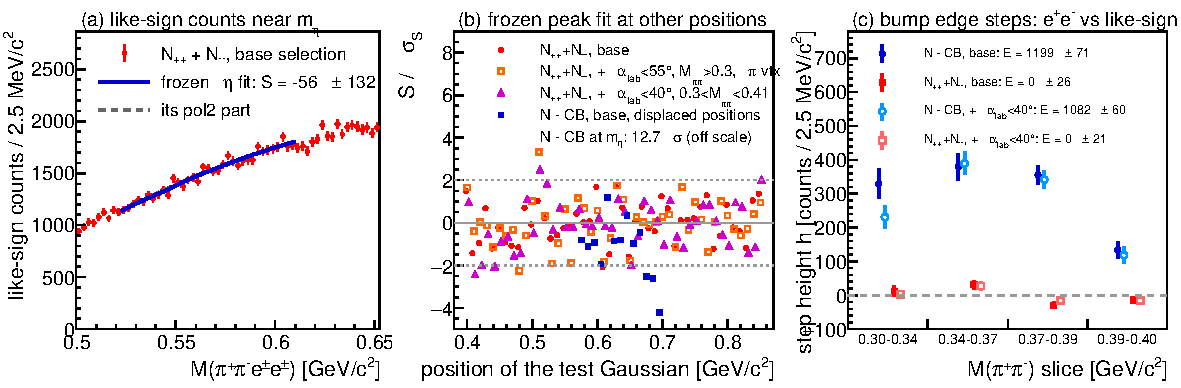
\includegraphics[width=\textwidth]{figs_exp/cb_null_cnt_plain.pdf}
\caption{\textbf{What it shows: the like-sign counts, from which the CB is made, contain no $\eta$ signal.} (a) The peak fit on
$N_{++}+N_{--}$ near the $\eta$ mass $m_\eta$: $S=-56\pm132$, against $4671\pm367$ in $N-\mathrm{CB}$. (b) $S/\sigma_S$ of the same fit moved
with its range to 46 positions in 0.40--0.85\,\GeVcc ($N_{++}+N_{--}$) and to 13 positions in 0.575--0.695\,\GeVcc ($N-\mathrm{CB}$, blue
squares; the lowest three reach the turnover of $N-\mathrm{CB}$ near 0.74\,\GeVcc); the $N-\mathrm{CB}$ value at $m_\eta$, 12.7, is off
scale. (c) Bump edge-step heights per \Mpipi slice on $N-\mathrm{CB}$ (blue) and on $N_{++}+N_{--}$ with the same fixed edges (red): the
like-sign counts show no edge ($0.5\pm25.6$ summed, printed rounded as $0\pm26$).
\emph{Selection:} data; \selbase; \selcb. (a): nothing more. (b) and (c): nothing more; \selpeaknom, and \selvtx; \selbumpnom (no
vertex-fit condition).
\emph{Words inside the figure:} ``base selection'' / ``base'' $=$ the base cuts; ``frozen $\eta$ fit'' / ``frozen peak fit'' $=$ the peak
fit; ``$\pi$ vtx'' $=$ \selvtx; $M_{\pi\pi}=\Mpipi$; ``test Gaussian'' $=$ the Gaussian of the peak fit moved to another mass. Counts,
not normalised to luminosity.}
\label{fig:res-cbnull}
\end{figure}

%----------------------------------------------------------------------
\subsection{The selection}
\label{sec:selection}
\textbf{The selection chosen on the simulation is as good as the best one tuned on the data} (Fig.~\ref{fig:res-selection}). Cuts
chosen on the same data on which they are measured favour upward fluctuations; this bias was measured on independent halves of the data.
The recommended selection raises the precision $F=S/\mathrm{stat}$ over the base cuts by $+1.35$ (from 12.7 to 14.1), as much as the
best automatic choice made blind on one half of the data and measured on the other ($+1.36$); the pion-distance cut alone gains $+1.00$.
The data-tuned peak selection gains $+1.57$ ($F=14.31$ against 14.09) but only about $+1.15$ once its tuning bias is removed. Most of the
gain comes from the two pion-vertex conditions (both pion tracks in the vertex fit, or both within 40\,mm of the vertex along the beam);
once one of them is in, the kinematic cuts do not improve $F$, and a cut on the \ee opening angle (above $2^\circ$) removes about 22\,\% of
the peak and never improves the precision. \emph{Status:} provisional.

\begin{figure}[tbp]
\captionsetup{margin=0pt}
\begin{minipage}[t]{0.485\textwidth}
\centering
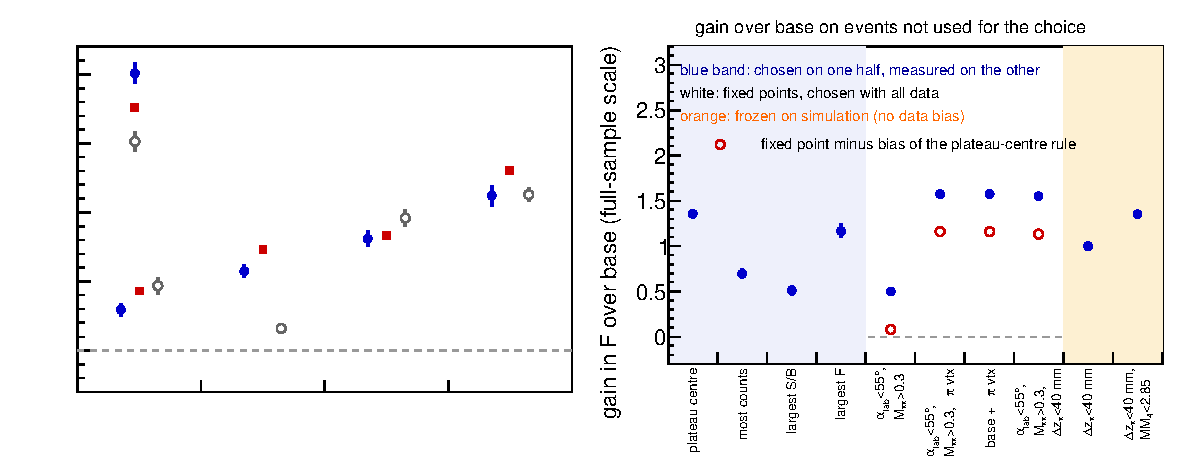
\includegraphics[width=\linewidth,trim=285 0 0 0,clip]{figs_exp/opt_bias_short.pdf}
\caption{\textbf{What it shows: the selection chosen on the simulation gains as much precision as the best blind choice on the data.}
Gain in $F=S/\mathrm{stat}$ (peak fit) over the base cuts alone, on events not used for the choice (full-sample scale). Blue band:
four automatic rules choose cuts on one half of the data and are measured on the other half (40 random halvings), from a grid of 840 cut
combinations: \alab below 40, 45, 50, 55, 60 or $65^\circ$ or no cut; \Mpipi above 0.30, 0.32 or 0.34\,\GeVcc or no cut; both pions, at
least one pion or no pion in the vertex fit; \dzpi below 20, 30, 40 or 60\,mm or no cut; $\MMfour<2.85$\,\GeVcc or no cut. Rules: the
plateau centre of a cut scan ($+1.36$; it chooses $\alab<55^\circ$, $\Mpipi>0.30$\,\GeVcc, at least one pion in the vertex fit and
$\dzpi<40$\,mm in 40 of the 80 halves; the other rules choose different cuts in different halves); the most counts in the peak window among the points within 1 of the largest $F$; the largest
$S/B$ among the same points; the largest $F$. The missing-mass cut is never chosen. White: fixed cut sets chosen with all data, among
them the data-tuned peak selection ($+1.57$); open red: the same minus the tuning bias measured for the plateau-centre rule (about
$+1.15$); the open red circle at the top left is the legend symbol. Orange: selections chosen on the simulation (recommended $+1.35$,
pion-distance cut alone $+1.00$).
\emph{Selection:} data; \selbase; the cuts of each point on top; peak fit as in Fig.~\ref{fig:fits}.
\emph{Words inside the figure:} ``base'' $=$ the base cuts; ``$\pi$ vtx'' $=$ \selvtx; $M_{\pi\pi}=\Mpipi$; $\mathrm{MM}_4=$ missing mass;
``frozen on simulation'' $=$ chosen on the simulation.}
\label{fig:res-selection}
\end{minipage}\hfill
\begin{minipage}[t]{0.485\textwidth}
\centering
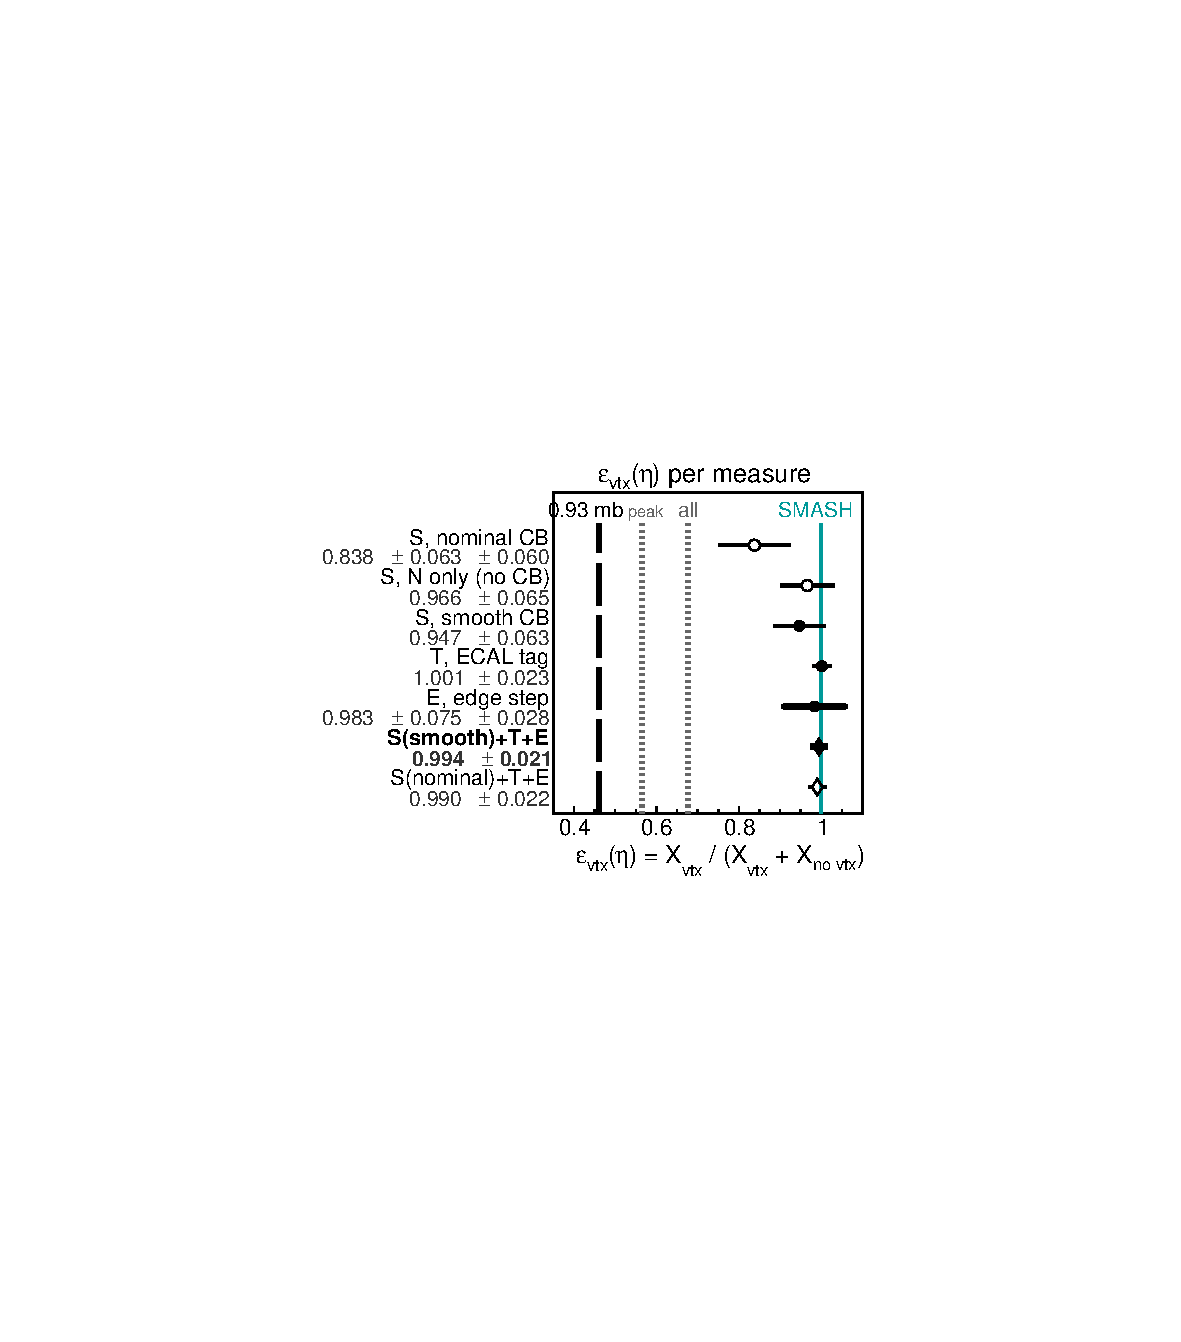
\includegraphics[width=\linewidth,trim=140 216 140 216,clip]{figs_exp/fix2_vtx_fig_cnt_crop.pdf}
\caption{\textbf{What it shows: every measure finds the $\eta$ in the counts kept by the event-vertex cut.} Share
$\varepsilon_{\mathrm{vtx}}$ of each $\eta$ measure in the counts with an event vertex: $S$ (peak fit) with the usual CB, without CB, and
with a smooth like-sign CB ($N_{++}$ and $N_{--}$ each fitted with a polynomial; used for the result); $T$, the ECAL-tagged $\eta$
(Section~\ref{sec:prod}); $E$, the bump edge step (thick bar: statistical error enlarged by 1.2; thin bar: with the model rms). Open
markers: not used for the result. The usual CB gives $0.838\pm0.063\pm0.060$ because the CB of the counts without a vertex has a dip at
the $\eta$ mass from a 2.4$\sigma$ downward fluctuation of their $e^+e^+$ counts; before CB subtraction these counts show no peak.
Combined ($S$ with the smooth CB, $T$, $E$): $0.994\pm0.021$ (0.990 with the usual CB). Vertical lines: simulation, 0.9997; survival of
the counts in the peak window (0.565) and of all counts (0.677), not $\eta$ efficiencies; 0.46, the share that would be needed for an
$\eta$ cross section of 0.93\,mb (a published HADES value at 3.5\,GeV) instead of the 0.43\,mb of Part~III.
\emph{Selection:} data, all 29 days read before any vertex requirement; \selptthree; \selpid; \selcor; \selall; no target-region cut;
whole events split into those with a reconstructed event vertex ($\vz>-500$\,mm) and those without (\vz set to $-1000$\,mm), each group
with its own CB from its own like-sign counts, $k=1$. $S$: peak fit as in Fig.~\ref{fig:fits}; $T$: ECAL photon tag as in
Section~\ref{sec:prod}; $E$: edge steps in the four \Mpipi slices 0.30--0.34, 0.34--0.37, 0.37--0.39 and 0.39--0.40\,\GeVcc as in
Fig.~\ref{fig:bump}.
\emph{Words inside the figure:} $X$ $=$ any of the measures; ``vtx'' / ``no vtx'' $=$ with / without an event vertex; ``nominal CB''
$=$ the usual CB; ``N only (no CB)'' $=$ no CB subtracted; ``SMASH'' $=$ simulation; ``peak'', ``all'' $=$ the survival lines;
``0.93\,mb'' $=$ the line at 0.46. Counts, not normalised to luminosity.}
\label{fig:res-vertex}
\end{minipage}
\end{figure}

%----------------------------------------------------------------------
\subsection{The event-vertex cut}
\label{sec:vertex}
\textbf{The event-vertex cut keeps the $\eta$} (Fig.~\ref{fig:res-vertex}). Only counts with a reconstructed event vertex
($\vz>-500$\,mm; the vertex finder needs at least two tracks in $-170<z<-30$\,mm) are kept; this removes 32\,\% of the \ee counts but
70--76\,\% of the like-sign counts. The removed counts hold no ECAL-tagged $\eta$ ($T=-4\pm77$, against 3297 in the kept counts;
the base cuts, a part of the kept counts, give 3314 with the code of the main analysis, a difference within the errors) and no bump edge ($E=21\pm96$ against 1241); the peak fit finds no significant $\eta$ there either ($263\pm324$ counts) once the CB of these counts is taken from smooth fits of their like-sign
spectra (the usual CB gives $0.838\pm0.063\pm0.060$ for the share kept, because the CB of the removed counts has a dip at the $\eta$ mass
from a 2.4$\sigma$ downward fluctuation of their $e^+e^+$ counts; before CB subtraction they show no peak). With three measures
combined the cut keeps $\varepsilon_{\mathrm{vtx}}=0.994\pm0.021$ of the $\eta$ (0.990 with the usual CB; simulation 0.9997). The survival of the counts (0.565 in
the peak window, 0.677 for all counts) is not an $\eta$ efficiency. The removed counts are mostly not p+p collisions in the hydrogen:
87\,\% of their pion pairs cross 8\,mm or more from the beam axis (35\,\% with a vertex), near $z\approx-200$\,mm, in front of the cell;
beam halo on the material there is a hypothesis, supported by the empty-target runs. A correction would raise the yields by
$0.6\pm2.1$\,\% (not applied). The like-sign counts peak at $\vz=-158.5$\,mm, just at the target-region cut $-160$\,mm: this peak is target
material (it is present in the empty-target runs). The cut $\vz>-160$\,mm keeps 0.93 of the \ee and 0.71--0.73 of the like-sign counts,
and there is no $\eta$ signal below $-160$\,mm. \emph{Status:} measured.

%----------------------------------------------------------------------
\subsection{Luminosity, stability and the target walls}
\label{sec:norm}
\textbf{Luminosity.} From elastic p+p scattering analysed without the START time, $L=6079.2\,\nbinv\pm6.9$\,\% for the 17\,557 analysed runs
(6080.5\,\nbinv for all runs); the yields include the factor 64/63 of the trigger bit (Section~\ref{sec:results}). Three one-sided effects,
not corrected, could make the yields up to about 11\,\% too low: the ratio 0.932 of the live fractions of PT3 and of PT2 (the trigger from
which $L$ is made), if it applies (yields up to $+7.3$\,\%); a trigger loss in sector~2 on days 034--044 ($+1.2$\,\% if corrected); and
events lost in the track reconstruction, one step of which still uses the START time ($+1.3$--1.6\,\% or $+2.2$--2.8\,\%). On day 045 the
elastic events show no sector-2 loss (PT2 $1.074\pm0.009$, PT3 $1.074\pm0.008$ of the clean-day ratio, against 0.65--0.76 and 0.92--0.98 on
days 041--044), so $L$ needs no correction there; the low sector-2 share of our counts on that day (efficiency $0.903\pm0.007$) is not
explained. \emph{Status:} the bookkeeping of $L$ is final; the absolute luminosity and the one-sided effects are provisional.

\textbf{Stability} (Fig.~\ref{fig:res-norm}). The count rates per luminosity scatter by 4.9\,\% rms per day (like-sign 13--14\,\%), in
steps between the beam periods, so the integrated yields carry $\pm5$\,\%. The $\eta$-peak yield per period is constant within its errors
($\chi^2/\mathrm{ndf}=1.4/3$). The steps follow the beam-halo level measured with the counts in front of the cell (correlation 0.93; a fit
with it leaves 1.7\,\% rms): an indication, not yet a proof. \emph{Status:} provisional.

\textbf{The target walls give a visible part of the counts but almost none of the $\eta$} (Fig.~\ref{fig:res-walls}). The luminosity is
for the liquid hydrogen only. 127 empty-target runs (days 034, 047 and 065), processed with the same programs and cuts and scaled to the
full-target runs of the same day with the counts in front of the cell, show that the walls (the Mylar windows of the cell and the material
around it) give $13.1\pm0.9$\,\% of the $N-\mathrm{CB}$ counts in 0.40--0.70\,\GeVcc with both pion tracks in the vertex fit, and
$19.0\pm1.1$\,\% with the base cuts alone (both raw). Corrected for the higher halo level of the three empty-target days, the share with
both pions in the vertex fit is 12.5\,\% in 0.40--0.70\,\GeVcc and 14.7\,\% in the bump and peak windows together (16.8\,\% there before the
correction). The share is plausible: in the target geometry the three Mylar windows (0.3\,mm in total) hold 11.9\,\% as many nucleons as the
hydrogen, so 5--12\,\% is expected if the production per nucleon scales between $A^{2/3}$ and $A$. But the walls carry almost none of the
$\eta$: in 12 vertex slices of the full data the $\eta$ per count in the walls is $r=0.07\pm0.30$ times that in the hydrogen (the
entrance-window slices alone, where 30--90\,\% of the counts are wall counts: $r=-0.27\pm0.34$), a wall share of the $\eta$ signal
$f_\eta=3^{+4}_{-3}$\,\%. A check with the simulated vertex shape of the hydrogen agrees: the share of the $\eta$ in the cell centre is
$0.566\pm0.045$ from $S$ and $0.571\pm0.024$ from $T$, against 0.577 for hydrogen alone; if the $\eta$ had the 16.8\,\% wall share of the
counts, it would be 0.497, excluded at 3.4$\sigma$. \emph{Meaning:} the visible $\eta$ yields of this report would be lower by
$3^{+4}_{-3}$\,\% if the walls were subtracted (Part~III multiplies its $\eta$ yields by 0.97); the wall share of the counts does not apply
to the $\eta$ yields, because the side bands and the background polynomial already remove the wall counts that do not peak.
\emph{Status:} measured.

\begin{figure}[tbp]
\captionsetup{margin=0pt}
\begin{minipage}[c]{0.60\textwidth}
\centering
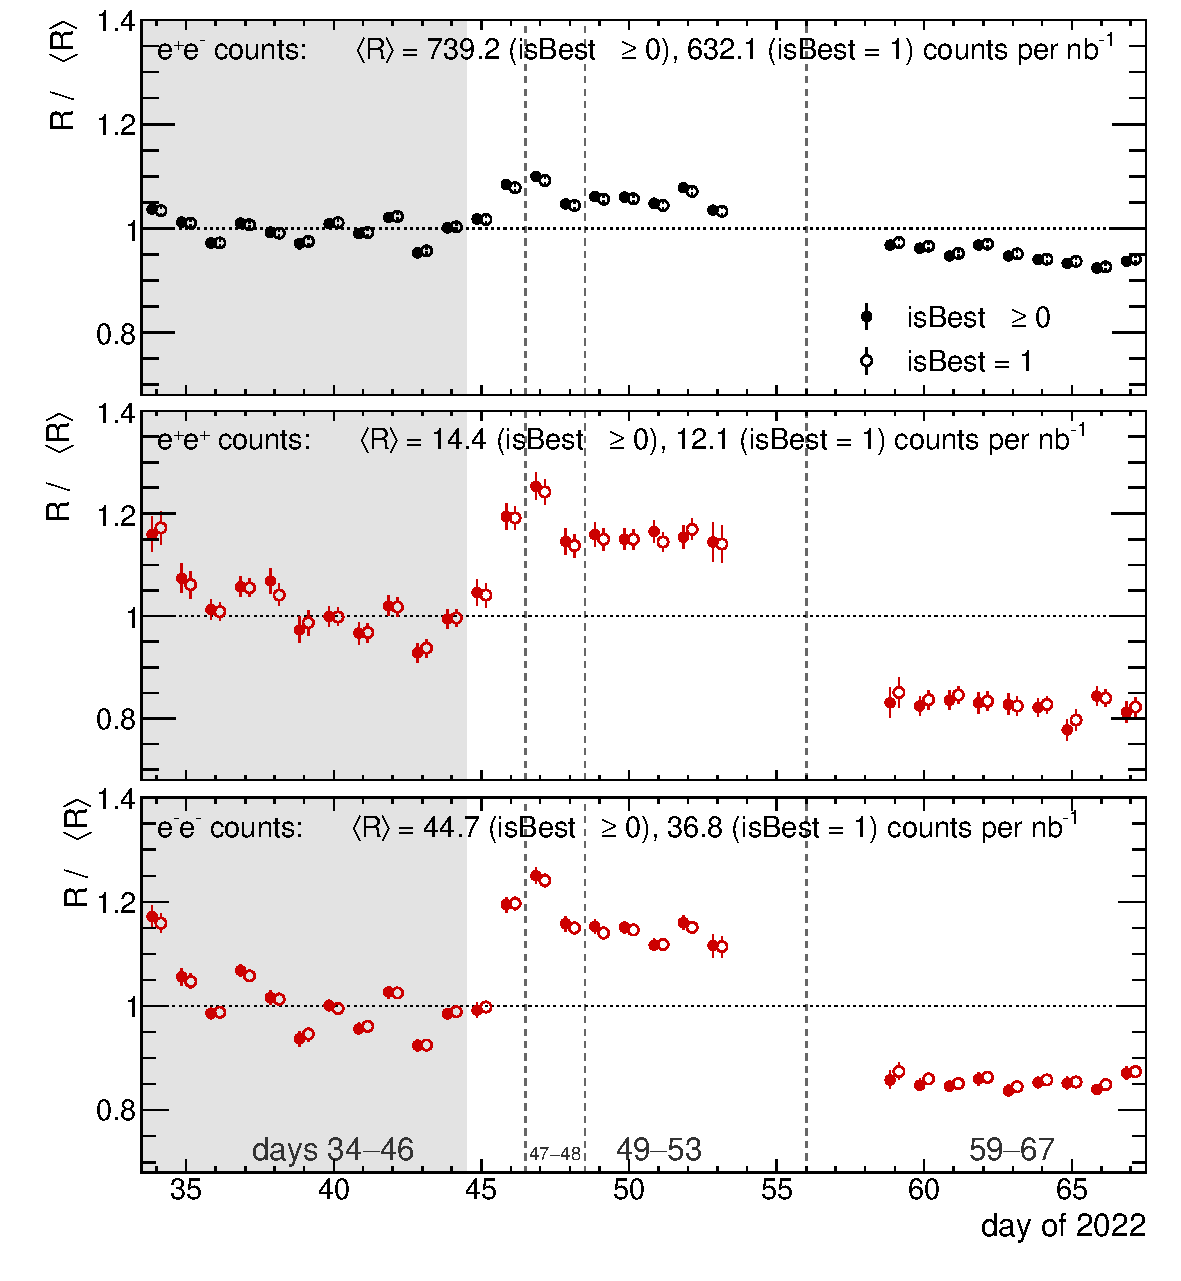
\includegraphics[width=\linewidth]{figs_exp/smp_rates_perday_cnt_plain2.pdf}
\end{minipage}\hfill
\begin{minipage}[c]{0.37\textwidth}
\caption{\textbf{What it shows: count rates per luminosity change in steps between the beam periods,} hence the $\pm5$\,\% period
normalisation. Rate per day $R=\text{counts}\times\frac{64}{63}/L$ relative to the luminosity-weighted mean $\langle R\rangle$, for \ee (top),
$e^+e^+$ (middle) and $e^-e^-$ counts (bottom), no CB subtracted; full markers: all stored combinations; open: best-ranked only; grey:
days 034--044, when sector~2 of the trigger lost events (a loss that $L$ does not correct); dashed: period boundaries. \ee: 4.9\,\% rms per
day (like-sign 13--14\,\%). $L$ from elastic scattering, 6079.2\,\nbinv $\pm6.9$\,\%.
\emph{Selection:} data; \selbase; all \Mfour, \Mee and \Mpipi.
\emph{Words inside the figure:} ``isBest $\ge0$'' / ``isBest $=1$'' $=$ all / best-ranked combinations; ``days 34--46'', ``47--48'',
``49--53'', ``59--67'' $=$ the beam periods.}
\label{fig:res-norm}
\end{minipage}
\end{figure}

\begin{figure}[tbp]
\centering
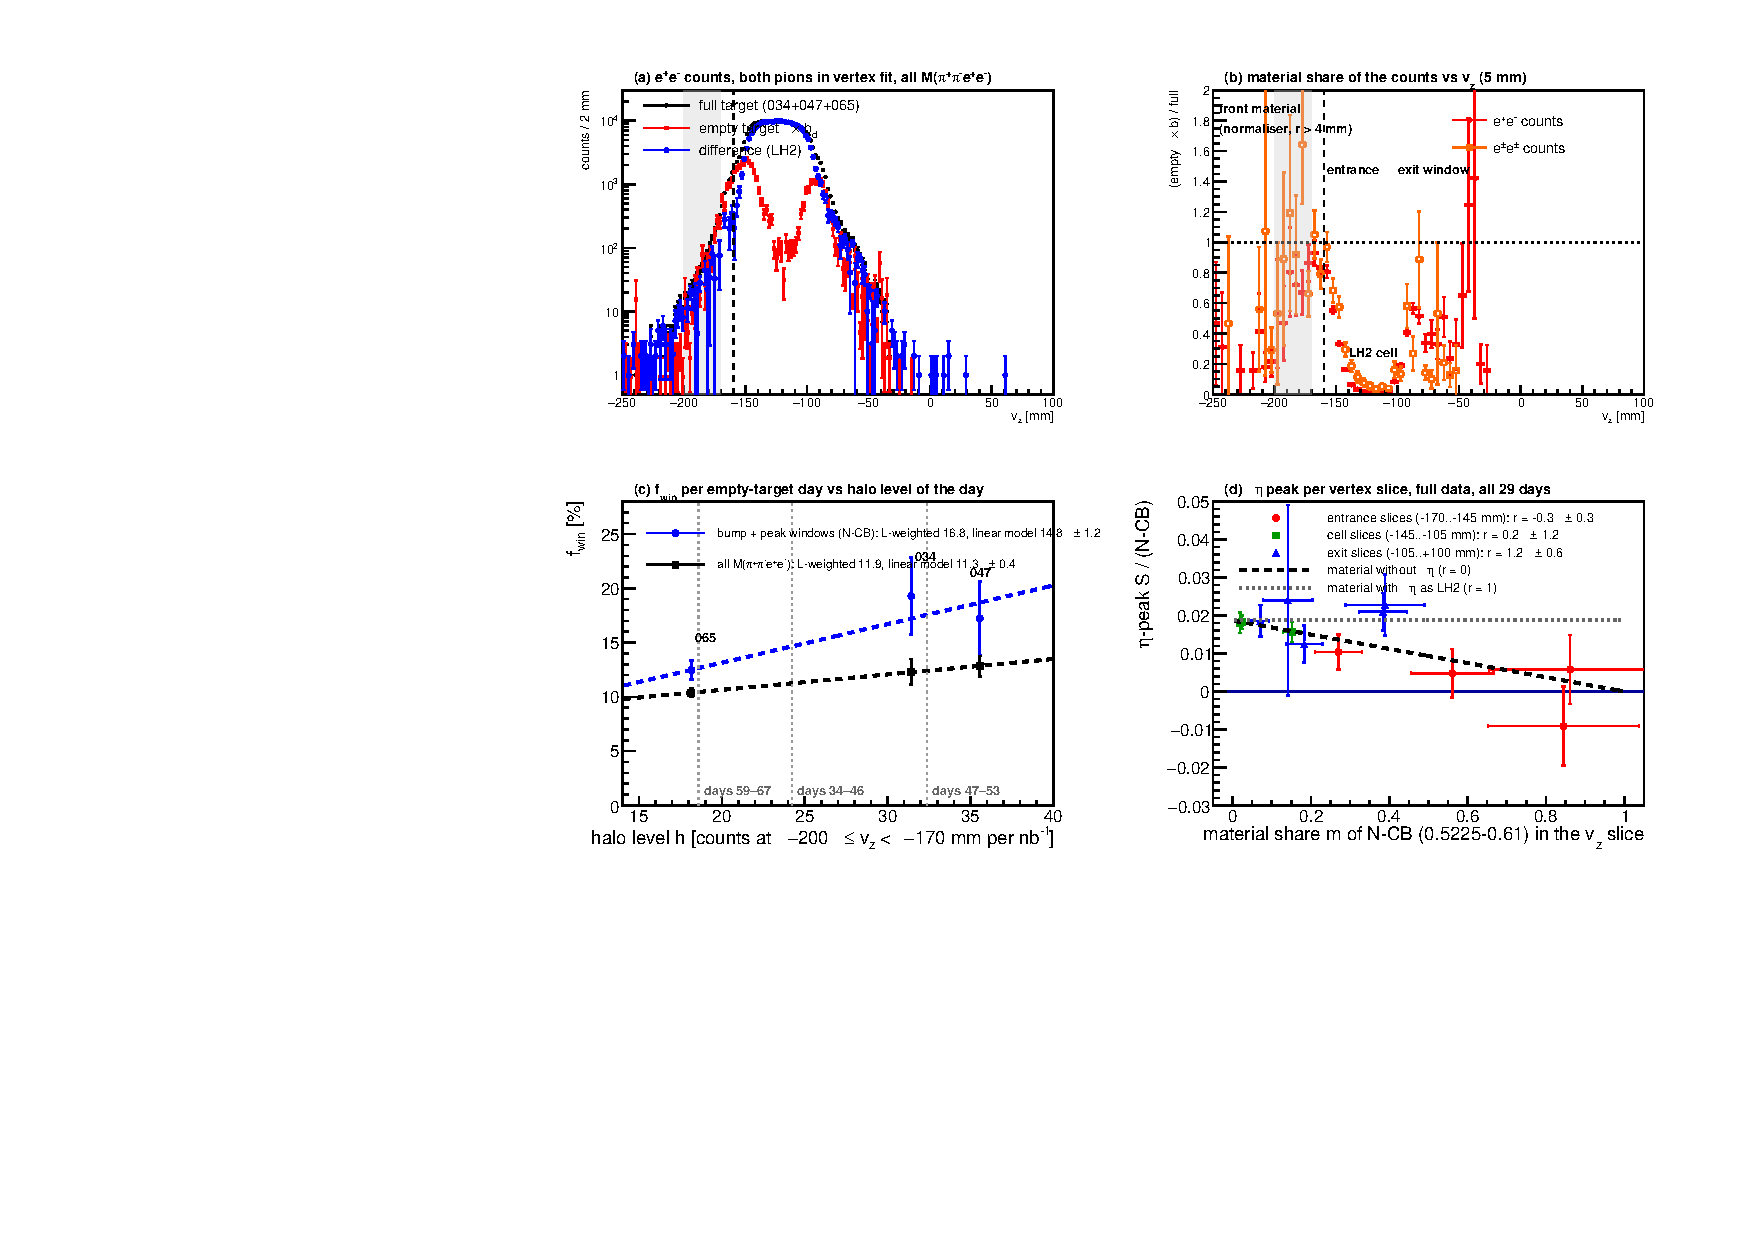
\includegraphics[width=\textwidth]{figs_all/vw2a_fig_cnt_plain.pdf}
\caption{\textbf{What it shows: the target walls give a visible part of the counts, but the $\eta$ signal does not come from them.}
Full-target runs of all 29 days and empty-target runs of days 034, 047, 065. (a) Event-vertex $z$ of the \ee counts, days 034 + 047 + 065:
full target (black), empty target scaled by the flux ratio of the same day (red), their difference, the hydrogen (blue). (b) Wall share of
the counts per 5\,mm slice of \vz: the walls dominate at the entrance ($\approx-150$\,mm) and the exit window ($\approx-90$\,mm); inside
the cell they give about 1\,\%. (c) Wall share of the $N-\mathrm{CB}$ counts per empty-target day (labels 065, 034, 047) against the
beam-halo level of that day: it follows the halo; dotted lines: the halo levels of the beam periods; at the luminosity-weighted halo
level the line drawn gives $14.8\pm1.2$\,\% instead of 16.8\,\% in the bump and peak windows (a separate halo correction gives
$14.7\pm1.1$\,\%). (d) $\eta$-peak content (peak fit in 0.5225--0.61\,\GeVcc) per $N-\mathrm{CB}$ count in each \vz slice against the
wall share of the slice; walls without $\eta$: dashed line, walls with $\eta$ like hydrogen: dotted line. The entrance slices (red),
with 30--90\,\% wall counts, fall to about zero ($r=-0.27\pm0.34$ for these slices alone, printed rounded); the exit-window slices (blue) are
consistent with the hydrogen rate ($r=1.21\pm0.64$); the fit of all slices gives $r=0.07\pm0.30$ and $f_\eta=3^{+4}_{-3}$\,\%.
\emph{Selection:} data; \selptthree; a reconstructed event vertex ($\vz>-500$\,mm) but no target-region cut in (a), (b) and (d), where
\vz is the variable (12 slices with the edges $-170$, $-160$, $-155$, $-150$, $-145$, $-135$, $-115$, $-105$, $-100$, $-95$, $-85$, $-60$ and
$+100$\,mm in (d)); \selpid; \selcor; \selall; \selvtx; all \Mfour in (a) and (b); (c) adds the target-region cut $\vz>-160$\,mm, all \Mfour
and the bump and peak windows together (0.4550--0.5225 and 0.53364--0.55416\,\GeVcc). Flux ratio of each day from the counts at
$-200\le\vz<-170$\,mm (beam halo, off the beam axis; no pion-vertex requirement there). \selcb.
\emph{Words inside the figure:} \fwin $=$ wall share of the $N-\mathrm{CB}$ counts; ``L-weighted 16.8'' and ``11.9'' $=$ the
luminosity-weighted wall shares before the halo correction, in the bump and peak windows together and in all \Mfour; ``linear model'' $=$
the line drawn; $b_d$ $=$ flux ratio of day $d$; LH2 $=$ liquid hydrogen; ``front material (normaliser, $r>4$\,mm)'' $=$ the region in
front of the cell where the flux ratio is measured, more than 4\,mm from the beam axis; $m$ $=$ wall share of the slice. Counts, not
normalised to luminosity.}
\label{fig:res-walls}
\end{figure}

%----------------------------------------------------------------------
\subsection{Reconstruction, particle identification and the ECAL tag}
\label{sec:prod}
\textbf{The reconstruction without the START time finds $1.38\pm0.17$ times the $\eta$-peak content of the earlier one}
(Fig.~\ref{fig:res-oldnew}), which measured velocities against the start time of the LGAD start detector (same days, same cuts, same fit;
the error treats the two samples as independent and is an upper bound): about 1.07 from events without an LGAD time (a luminosity effect)
times 1.29--1.33 more signal in the same events, a loss of the earlier, start-time based method; in the simulation, which has a perfect
start time, the two reconstructions differ only by 1.04. \emph{Status:} cross-check. \textbf{Particle identification} uses \betanew,
computed from the time differences of the tracks of each combination, so a START error cancels; the pion bands of the data are
30--50\,\% wider than in the simulation; protons fill the \pip slot above 1.9\,\GeVc (in 3.15\,\% of all counts, 0.15\,\% in the peak
window). Counts without an energy-loss-corrected \pim momentum (0.62\,\% of the \ee counts, \pim below $16^\circ$) are dropped.
\textbf{ECAL tag.} When the electromagnetic calorimeter (ECAL) also finds the photon, $\eta\to\pipi\piz$ is reconstructed in full and
appears as a clean third $\eta$ peak in $m_{5c}=M(\ppee\gamma)$, with the photon energy rescaled so that $M(\ee\gamma)$ equals the \piz
mass. The photon is a cluster identified as a photon by the ECAL with $0.8<\beta<1.2$ and energy above 100\,MeV (of up to three such
photons the one with $M(\ee\gamma)$ closest to 0.140\,\GeVcc), with $0.119\le M(\ee\gamma)<0.173$\,\GeVcc and $\Mee<0.10$\,\GeVcc; $T$ is the
content of a fixed Gaussian (0.5463\,\GeVcc, 6.2\,\MeVcc) plus a second-order polynomial fitted to $N-\mathrm{CB}$ in $m_{5c}=0.49$--0.62\,\GeVcc.
With the base cuts $T=3314\pm105\pm124$ counts ($Y_T=0.554\pm0.018$ visible counts per \nbinv), a check of the other two signals;
$S/T=1.409\pm0.119\pm0.15$, not corrected for the different acceptances. The ECAL sector at azimuth 63--117$^\circ$ is off and 8 further
modules are dead, the same map as in the simulation; the photon energy is about 17\,\% too high, so the 100\,MeV cluster cut acts near
85\,MeV of true energy; the cut $0.8<\beta<1.2$ uses the START time, so the 6.4\,\% of the counts without a START hit are tagged at only
0.69--0.80 of the normal rate, which costs $T$ 1.4--2.3\,\%. These findings matter only when $T$ is compared with a simulated tag; the
measured $T$ stands as it is. \emph{Status:} $T$ final, the ECAL findings measured.

\begin{figure}[tbp]
\captionsetup{margin=0pt}
\begin{minipage}[c]{0.36\textwidth}
\centering
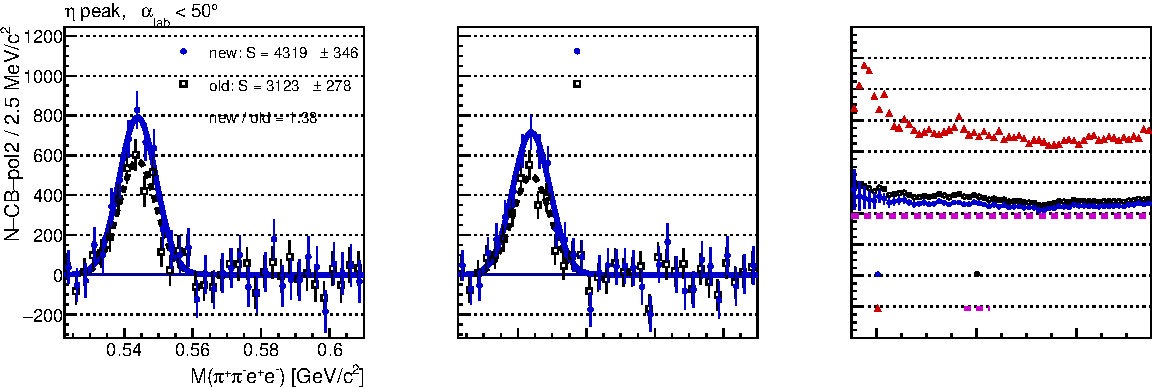
\includegraphics[width=\linewidth,trim=0 0 368 0,clip]{figs_exp/res_oldnew_peak_short.pdf}
\end{minipage}\hfill
\begin{minipage}[c]{0.60\textwidth}
\caption{\textbf{What it shows: the reconstruction without the START time holds 1.38 times the $\eta$ content of the earlier one.}
$N-\mathrm{CB}$ minus the polynomial of the peak fit, earlier reconstruction (velocities against the LGAD start time, open squares) and
the one used in this report (\betanew, blue), the same 29 days; CB with $k=1$; each combination counted once in both. Printed: $S$ of each
and the ratio $1.38\pm0.17$ (the error is an upper bound); the simulation changes only by 1.04.
\emph{Selection:} data; the same cuts for both reconstructions, those of their first comparison: \selptthree; a reconstructed event
vertex ($\vz>-500$\,mm) but no target-region cut; each reconstruction with its own particle identification (\betanew, or velocities
measured against the LGAD start time); \selcor; \selall; $\alab<50^\circ$. Peak fit as in Fig.~\ref{fig:fits}.
\emph{Words inside the figure:} ``new'' / ``old'' $=$ the reconstruction of this report / the earlier one; pol2 $=$ second-order
polynomial. Counts, not normalised to luminosity.}
\label{fig:res-oldnew}
\end{minipage}
\end{figure}

\begin{figure}[tbp]
\captionsetup{margin=0pt}
\begin{minipage}[t]{0.485\textwidth}
\centering
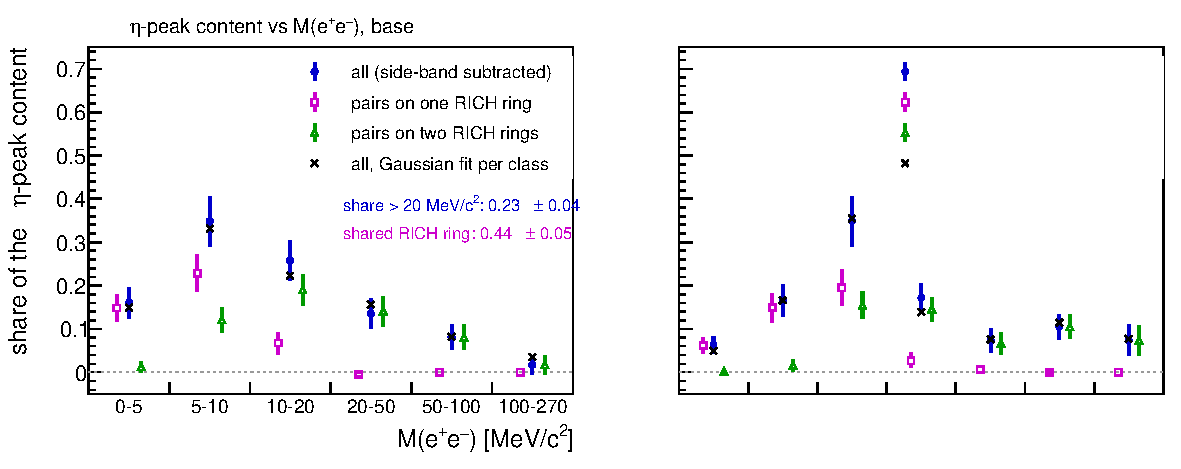
\includegraphics[width=0.94\linewidth,trim=0 0 283 0,clip]{figs_exp/res_mee_content_short.pdf}
\caption{\textbf{What it shows: close pairs dominate the $\eta$ peak; only 0.23 of it lies above $\Mee=20$\,\MeVcc.} Share of the
$\eta$-peak content per \Mee band (0--5, 5--10, 10--20, 20--50, 50--100, 100--270\,\MeVcc); blue: side-band subtraction in \Mfour
(stat $\oplus$ model); magenta / green: pairs on one shared / on two RICH rings; crosses: the peak fit of each band alone. Share above
20\,\MeVcc: $0.23\pm0.04\,(\mathrm{stat})\pm0.05\,(\mathrm{method})$. The direct-decay shape is not drawn: from the 20--50\,\MeVcc band
and equal content per logarithmic \Mee interval it gives about 490 counts in each of 5--10 and 10--20\,\MeVcc, where the data hold 1673 and
1236 (an excess of about 40\,\% of the peak).
\emph{Selection:} data; \selbase; peak window 0.53364--0.55416\,\GeVcc, side bands 0.5225--0.53364 and 0.55416--0.56530\,\GeVcc;
CB of each \Mee band from its own like-sign counts, $k=1$.
\emph{Words inside the figure:} ``base'' $=$ the base cuts; ``class'' $=$ \Mee band; ``Gaussian fit'' $=$ the peak fit. Not normalised
to luminosity.}
\label{fig:res-mee}
\end{minipage}\hfill
\begin{minipage}[t]{0.485\textwidth}
\centering
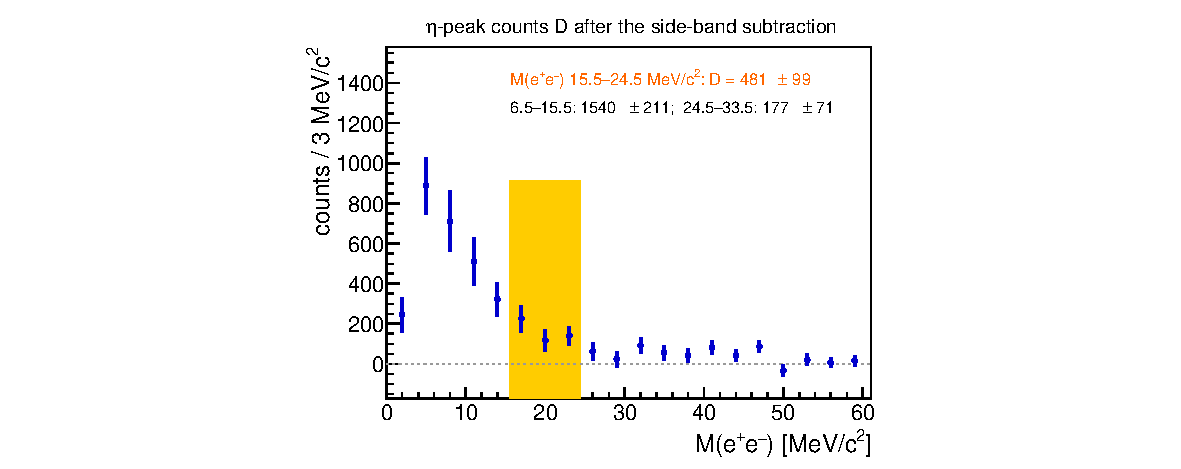
\includegraphics[width=0.94\linewidth,trim=140.5 0 140.5 0,clip]{figs_exp/res_x17_window_cnt_crop.pdf}
\caption{\textbf{What it shows: the X17 search band (orange) holds as many $\eta$ counts as its \Mee neighbours predict.}
$\eta$-peak counts $D$ after the side-band subtraction, per 3\,\MeVcc of \Mee. In 15.5--24.5\,\MeVcc $D=481\pm99$, against $522\pm111$
from the log-linear interpolation (the geometric mean) of the neighbouring bands 6.5--15.5 and 24.5--33.5\,\MeVcc (values printed in the
figure). No limit is derived (it needs the simulated X17 efficiency).
\emph{Selection:} data; \selbase; \selvtx; the data peak window 0.53364--0.55416\,\GeVcc, side bands 0.5225--0.53364 and
0.55416--0.56530\,\GeVcc (Part~III searches in the wider window 0.5312--0.5566\,\GeVcc, Table~\ref{tab:sel}); CB of each \Mee bin from
the like-sign counts of that bin, $k=1$. Not normalised to luminosity.}
\label{fig:res-x17}
\end{minipage}
\end{figure}

%----------------------------------------------------------------------
\subsection{Content of the peak and the X17 search band}
\label{sec:mee}
\textbf{Inside the peak, close pairs dominate} (Fig.~\ref{fig:res-mee}). Split into six \Mee bands with a side-band subtraction in each,
$0.23\pm0.04\,(\mathrm{stat})\pm0.05\,(\mathrm{method})$ of the peak lies above $\Mee=20$\,\MeVcc (the same with either side band alone),
and $0.772\pm0.037$ has an opening angle above $2^\circ$. Between 5 and 20\,\MeVcc the data hold about $1900\pm400$ counts (about 40\,\% of
the peak) more than a direct decay alone would give: taking the 650 counts of the 20--50\,\MeVcc band as pure direct decay and equal
content per logarithmic \Mee interval (Kroll--Wada, roughly $1/\Mee$), a direct decay would put about 490 counts into each of the bands
5--10 and 10--20\,\MeVcc, where the data hold 1673 and 1236. \emph{Meaning:} this would fit $\eta\to\pipi\gamma$ with the photon converted
in the material, but the data alone do not prove it (equal acceptance assumed); a shared RICH ring ($0.439\pm0.045$ of the peak) follows
the opening angle and does not tell the two origins apart. \emph{Status:} provisional; the split into direct decay and conversion is not
determined without the simulation.

\textbf{Nothing unusual where an X17 boson would appear} (Fig.~\ref{fig:res-x17}). A hypothetical 17\,\MeVcc boson from $\eta\to\pipi X17$,
$X17\to\ee$ would show in the $\eta$-peak counts with $15.5\le\Mee<24.5$\,\MeVcc. In the peak window ($N=5258$ counts, CB $=101.7$) the
side-band subtraction leaves $D=481\pm99$ $\eta$ counts, against $522\pm111$ from a log-linear interpolation (the geometric mean) of the
neighbouring \Mee bands, 6.5--15.5\,\MeVcc ($1540\pm211$) and 24.5--33.5\,\MeVcc ($177\pm71$). The peak fit of the same band without any
\Mfour window gives $S=440\pm92\pm60$ (Table~\ref{tab:main}), the content of the whole Gaussian, which agrees with $D$ once $D$ is scaled
from the window to the whole peak ($541\pm111$). A limit needs the simulated X17 efficiency and is not determined here; Part~III gives
$\mathrm{BR}(\eta\to\pipi X17)\,\mathrm{BR}(X17\to\ee)<3.16\times10^{-5}$ at 17\,\MeVcc (90\,\% CL$_s$, with the PDG 2026 value of
$\mathrm{BR}(\eta\to\ppee)$). \emph{Status:} cross-check.


%----------------------------------------------------------------------
\subsection{The numbers in one place}
\label{sec:mainnum}
% not a float: the parts (a) and (b) are two boxes that may fall on different pages
\par\noindent\begin{minipage}{\textwidth}\centering
\captionsetup{type=table}
\caption{\textbf{The main numbers} of the data (symbols: Section~\ref{sec:nota}). (a) $\eta$-peak content $S\pm$stat$\pm$model (peak
fit) and visible yield $Y=S\times\frac{64}{63}/L$ [visible counts per \nbinv] for the selections of Table~\ref{tab:sel} (all with the
base cuts); variants with only the best-ranked combination of each event and with an \ee opening angle above $2^\circ$ (both together are
in the full report); CB$/N$ in the peak window 0.53364--0.55416\,\GeVcc. The last row is the $\eta$ content of the X17 search band, without
an \Mfour window. (b) Other results. Errors and conventions: notes below.}
\label{tab:main}
\footnotesize
\setlength{\tabcolsep}{3pt}
(a)\\[0.2em]
\begin{tabularx}{\textwidth}{@{}L r r r r r@{}}
\toprule
 & \multicolumn{2}{c}{all combinations} & all, OA$>2^\circ$ & best-ranked only & \\
Cuts on top of the base cuts & $S$ & $Y$ & $S$ & $S$ & CB$/N$ \\
\midrule
$\dzpi<40$\,mm, $\MMfour<2.85$\,\GeVcc (recommended) & $4364\pm310\pm477$ & $0.729\pm0.052\pm0.080$ & $3302\pm274\pm366$ & $4061\pm281\pm470$ & 0.072 \\
$\dzpi<40$\,mm (pion-distance cut alone) & $4492\pm327\pm423$ & $0.751\pm0.055\pm0.071$ & $3460\pm290\pm325$ & $4112\pm296\pm391$ & 0.076 \\
none (base cuts alone $=$ bump edge selection) & $4671\pm367\pm453$ & $0.780\pm0.061\pm0.076$ & $3632\pm328\pm378$ & $4199\pm330\pm414$ & 0.103 \\
$\alab<55^\circ$, $\Mpipi>0.30$\,\GeVcc, both pions in the vertex fit (data-tuned) & $3949\pm276\pm373$ & $0.660\pm0.046\pm0.062$ & $3076\pm242\pm300$ & $3602\pm252\pm341$ & 0.055 \\
both pions in the vertex fit, $15.5\le\Mee<24.5$\,\MeVcc (X17 search band) & $440\pm92\pm60$ & $0.073\pm0.015\pm0.010$ & $441\pm92\pm58$ & $368\pm84\pm59$ & 0.019 \\
\bottomrule
\end{tabularx}
\end{minipage}

\vspace{0.4em}
{\footnotesize\setlength{\tabcolsep}{3pt}\setlength{\LTpre}{0pt}\setlength{\LTpost}{0pt}
\begin{longtable}{@{}>{\raggedright\arraybackslash}p{5.4cm} >{\raggedright\arraybackslash}p{\dimexpr\textwidth-5.4cm-2\tabcolsep\relax}@{}}
\multicolumn{2}{c}{(b)} \\
\toprule
Quantity & Value \\
\midrule
\endfirsthead
\multicolumn{2}{@{}l}{\emph{Table~\ref{tab:main}(b), continued}} \\
\toprule
Quantity & Value \\
\midrule
\endhead
bump edge-step sum $E$, base cuts alone (counts per 2.5\,\MeVcc) & $1199\pm71\pm287$; OA$>2^\circ$: $898\pm64\pm160$; best-ranked only: $1050\pm64\pm217$ \\
$E$, data-tuned bump selection ($\alab<40^\circ$, $0.30<\Mpipi<0.41$\,\GeVcc, both pions in the vertex fit) & $1004\pm51\pm244$$^{\ast}$; OA$>2^\circ$: $746\pm44\pm220$; best-ranked only: $884\pm46\pm247$ \\
bump edge position / $\eta$-peak mass scale & $0.9927\pm0.0013$ / $0.9927\pm0.0009$: the edge sits where $\eta\to\pipi\piz$ puts it \\
step at $u=0$, $h_u$ (both pions in the vertex fit, $0.30\le\Mpipi<0.40$\,\GeVcc, $\Mee<135$\,\MeVcc) & $1308\pm62$ counts per 2.5\,\MeVcc,
   21$\sigma$, data only; width free $1271\pm85$ ($\sigma_u=6.3\pm0.7$\,\MeVcc); Gaussian peak term from the data $1217\pm66$; Part~III
   (simulated peak shape) $1305\pm62$; the difference is the tail of the $\eta$ peak (about 50 counts), whose size the data cannot fix
   ($t=0.3\pm1.0$; Part~III uses the simulated tail with a $\pm50$\,\% uncertainty, $t=1\pm0.5$), and the positions of the peak counts
   (about 40 counts) \\
like-sign counts in $u$ (counts per 2.5\,\MeVcc) & $e^+e^+$ $2.1\pm6.5$; $e^-e^-$ $73.5\pm15.7$ (4.7$\sigma$); at $\Mee\ge90$\,\MeVcc $7.3\pm4.3$ / $57.0\pm9.1$:
   pairs from the two \piz photons; 39 counts (3\,\%) of $h_u$ enter through the CB, as they should \\
ECAL-tagged $\eta$ $T$, base cuts alone & $3314\pm105\pm124$, $Y_T=0.554\pm0.018$ visible counts per \nbinv; OA$>2^\circ$: $2506\pm93\pm98$;
   best-ranked only: $2850\pm96\pm116$; with both pions in the vertex fit: $3090\pm94$; the counts without a START hit are tagged at
   0.69--0.80 of the normal rate, which costs $T$ 1.4--2.3\,\% \\
$S/T$, base cuts alone (uncorrected) & $1.409\pm0.119\pm0.15$; best-ranked only: $1.474\pm0.126\pm0.16$; OA$>2^\circ$: $1.449\pm0.142\pm0.16$ \\
mass scales & \Mfour: $0.9927\pm0.0009$ ($0.54388/0.547862$); \Mpipi (from K$^0_S\to\pipi$): $0.99691\pm0.00036$ \\
event-vertex cut, share of the $\eta$ kept & $\varepsilon_{\mathrm{vtx}}=0.994\pm0.021$ (0.990 with the usual CB); correction $+0.6\pm2.1$\,\%, not applied \\
peak content with $\Mee>20$\,\MeVcc & $0.23\pm0.04\,(\mathrm{stat})\pm0.05\,(\mathrm{method})$; opening angle above $2^\circ$: $0.772\pm0.037$; one RICH ring $0.439\pm0.045$ \\
X17 search band in the peak window (both pions in the vertex fit) & $D=481\pm99$ counts; log-linear interpolation from the neighbouring \Mee bands $522\pm111$; no limit derived \\
$\eta$-peak yield per period & $\chi^2/\mathrm{ndf}=1.4/3$ (base cuts alone), 1.6/3 (data-tuned peak selection) \\
target walls (empty target) & $13.1\pm0.9$\,\% of $N-\mathrm{CB}$, 0.40--0.70\,\GeVcc (both pions in the vertex fit; base cuts alone $19.0\pm1.1$\,\% raw); $\eta$ share $f_\eta=3^{+4}_{-3}$\,\% (not subtracted) \\
sector~2, elastic events (PT2 / PT3) & days 041--044: 0.65--0.76 / 0.92--0.98 of the clean-day ratio; day 045: $1.074\pm0.009$ / $1.074\pm0.008$: $L$ right on day 045 \\
\bottomrule
\end{longtable}
\addtocounter{table}{-1}% the longtable is part (b) of Table tab:main: no own number
}

{\raggedright\footnotesize Notes. stat: fit error (per-count Poisson errors; confirmed with independent halves of the data for $S$ and by a
bootstrap for $E$, 0.98--1.04 of the fit error); model: rms over the fit variations that pass a $\chi^2$ probability above 0.05 (for $S$: 90
of 144 for the recommended selection). All combinations unless stated; CB with $k=1$; luminosity $\pm6.9$\,\% and the one-sided effects
(up to $+11$\,\%) not included; nothing is corrected for acceptance or efficiency.
$^{\ast}$\,Lower limit of the model error: the slice 0.39--0.40\,\GeVcc fails the $\chi^2$-probability condition in the standard fit
($\chi^2/\mathrm{ndf}=42.8/22$) and in all 18 variations, so its spread is undefined (counted as 0).\par}
\vspace{0.5em}

\floatbarrier

%======================================================================
\section{What is not determined here, and what stays open}
\label{sec:open}
%======================================================================
\inshort{The efficiencies, the bump yield and the X17 limit need the simulation (Part~III has since measured them); the luminosity side,
the CB normalisation and a few features of the data stay open.}

\begin{itemize}
\item \textbf{Needs the simulation:} the efficiencies of the selections (both pions in the vertex fit, \dzpi, the missing-mass cut, whose
      simulation was made at a beam energy of 4500\,MeV while the data kinematics use 4530\,MeV, the particle identification with the
      wider data bands, and the requirement of energy-loss-corrected momenta for all four tracks; the event-vertex cut is measured in the
      data, $0.994\pm0.021$), the bump yield, the conversion parts of both the peak ($\eta\to\pipi\gamma$) and the bump ($\piz\to\gamma\gamma$),
      which do not cancel in the peak/bump ratio, the split into direct decay and conversion, and the X17 limit. Part~III has since measured,
      with the SMASH simulation: the bump from the step in $u$, $0.426\pm0.020\pm0.034\pm0.030$ times the SMASH prediction, with the
      per-slice edge as a cross-check, $0.423\pm0.023\pm0.038\pm0.048$; the X17 limit $3.16\times10^{-5}$ (90\,\% CL$_s$, PDG 2026); and
      $\sigma(pp\to\eta X)=0.43\pm0.17\,(\mathrm{measurement})\,^{+0.08}_{-0.03}\,(\mathrm{model})$\,mb, preliminary because the make-up of
      the peak is still open. The ECAL-tagged $\eta$, $T$, is the bump reconstructed in full with the ECAL photon (about 12\,\% of the bump);
      Part~III compares it with the bump measurement times the simulated tag: data over expectation $1.16\pm0.21$ with the simulated photon
      energy scale and $0.84\pm0.15$ with a data-like one. Before this can be a measurement it needs the photon energy scale and
      resolution, the module efficiency, a photon cut without START and at least 10 times more simulated $\eta\to\pipi\piz$. The reading
      ``about 40\,\% conversions'' in the peak stays provisional: whether the data lose close \ee pairs more than the simulation is to be
      tested in a separate analysis (efficiency of \ee pairs with an opening angle of 0--6$^\circ$ in data and simulation, from \piz, $\eta$
      and $\omega$ Dalitz decays with the ECAL photon).
\item \textbf{Luminosity side:} whether the PT3 live fraction applies (one-sided, $-6.8$\,\% on $L$); the sector-2 loss in the trigger
      efficiency; the events lost in the track reconstruction (1.3--1.6\,\% or 2.2--2.8\,\%); the vertex condition of the elastic
      luminosity (not checked: about 1\,\% on $L$ if none, several per cent possible with the vertex of the reconstruction); for the target
      walls, the normalisation with the halo counts ($-12/+6$\,\% of the wall share of the counts), the timing of the day-034 and day-047
      empty runs, and the nucleon-count expectation of 5--12\,\% for the $\eta$, only partly covered by $f_\eta=3^{+4}_{-3}$\,\% (12\,\% lies
      at 2.3$\sigma$).
\item \textbf{CB:} $k=1$ is a convention, with the event-mixing factor as a systematic variant; its normalisation cannot be checked with
      data alone. In narrow \Mee bands the geometric mean of few like-sign counts is biased low: in the X17 search band (peak window) the
      CB is 101.7 counts as the per-cell geometric mean of this report ($N_{++}=14$), 112 as one geometric mean over the whole window, or
      $171\pm6$ with one like-sign share per 50\,\MeVcc band of \Mee, as in Part~III (the 124 of Table~\ref{tab:sel} belongs to the wider
      search window); the side-band numbers $D$ should be insensitive (not evaluated).
\item \textbf{Fit model:} the width of the fixed Gaussian dominates; the peak position is not varied (free fits move by $\pm0.6$\,\MeVcc);
      the fake peak content of the missing-mass cut depends on how the smooth spectrum is modelled ($+48\pm27$ or $+83\pm26$ counts for
      the recommended selection); the step in $u$ depends by up to 7\,\% on the tail of the $\eta$ peak, whose size the data cannot fix.
\item \textbf{Unexplained:} $E$ differs between two independent halves of the data by $-2.35\sigma$ (about $-2.4\sigma$ with bootstrap
      errors; 40 random halvings show no general asymmetry); whether the day-to-day steps of the count rates are fully the beam halo on the
      walls and the holder (if a per-day test confirms it, the $\pm5$\,\% could be reduced); why neither the counts without a vertex nor
      the entrance-window counts hold measurable $\eta$ (walls: $r=0.07\pm0.30$; exit-window slices alone $r=1.21\pm0.64$), although p+A
      collisions make $\eta$ mesons; the turnover of $N-\mathrm{CB}$ near 0.74\,\GeVcc (most likely the $\omega\to\pipi\piz$,
      $\piz\to\ee\gamma$ edge); the low sector-2 share of the counts on day 045 while the elastic events show none.
\end{itemize}

%======================================================================
\section{Symbols}
\label{sec:nota}
%======================================================================
{\footnotesize
\setlength{\tabcolsep}{4pt}
\renewcommand{\arraystretch}{1.08}
\begin{longtable}{@{}>{\raggedright\arraybackslash}p{3.3cm} >{\raggedright\arraybackslash}p{\dimexpr\textwidth-3.3cm-2\tabcolsep\relax}@{}}
\caption{\textbf{Symbols and words} used in this summary. A count is one stored \pip\pim$e^+e^-$ combination of four tracks; an event can
give more than one count.}
\label{tab:nota}\\
\toprule
\multicolumn{2}{@{}l}{\textbf{Samples and normalisation}} \\
all combinations / best-ranked & all stored combinations of an event (used for every result) / only the combination ranked best by the $\chi^2$ of its times of flight \\
$N$, $N_{++}$, $N_{--}$ & counts of \ppee and of the like-sign combinations $\pipi e^+e^+$ and $\pipi e^-e^-$ \\
PT3, PT2, 64/63 & PT3: the main reaction trigger, at least two sectors with an inner-TOF hit in coincidence with TOF or RPC and at
   least three inner-TOF paddles hit (trigger bit 8192); PT2: minimum bias, at least one such sector, downscaled by 64, the trigger from
   which $L$ is made; bit 8192 holds 63/64 of the PT3 events \\
START, LGAD & start-time detector in front of the target (LGAD sensors); this analysis does not use its time \\
\vz & $z$ of the reconstructed event vertex ($-1000$\,mm when the vertex finder found fewer than two tracks) \\
$L$ & luminosity from elastic scattering (analysed without the START time) of the 17\,557 analysed runs, 6079.2\,\nbinv $\pm6.9$\,\% \\
$Y$, $Y_T$ & visible yield $S\times\frac{64}{63}/L$ (or the same for $T$) in visible counts per \nbinv; not a cross section \\
$\varepsilon_{\mathrm{vtx}}$ & share of the $\eta$ kept by the event-vertex cut $\vz>-500$\,mm \\
\fwin, \feta & share of the target walls (empty-target runs) in the $N-\mathrm{CB}$ counts of a window; in the $\eta$ signal ($3^{+4}_{-3}$\,\%) \\
$r$ & $\eta$ per count in the walls over $\eta$ per count in the hydrogen \\
halo level & counts at $-200\le\vz<-170$\,mm (beam halo on material in front of the cell) per \nbinv \\
\midrule
\multicolumn{2}{@{}l}{\textbf{Selection}} \\
base cuts & \selbase \\
\betanew & START-free velocity from the time differences of the tracks of a combination \\
\Mfour, \Mee, \Mpipi, OA & invariant masses of \ppee, of the \ee pair and of the \pipi pair; opening angle of $e^+$ and $e^-$ \\
\dzpi & largest distance along the beam of the two pion tracks (closest approach to the beam axis) from the event vertex \\
\MMfour & missing mass of \ppee (beam + target $-$ \ppee), beam kinetic energy 4530\,MeV \\
\alab & angle between the \pipi and the \ee momenta in the laboratory \\
peak / bump window & \Mfour 0.53364--0.55416 / 0.4550--0.5225\,\GeVcc (data mass scale) \\
side bands & \Mfour 0.5225--0.53364 and 0.55416--0.56530\,\GeVcc \\
\midrule
\multicolumn{2}{@{}l}{\textbf{Background and signal measures}} \\
CB, $k$ & combinatorial background $k\cdot2\sqrt{N_{++}N_{--}}$ per 10\,\MeVcc of \Mfour; convention $k=1$ \\
peak fit, $S$ & fit of $N-\mathrm{CB}$ with a Gaussian fixed at 0.5439\,\GeVcc, width 5.4\,\MeVcc, plus a second-order polynomial in
   0.5225--0.6100\,\GeVcc; $S$ its Gaussian content \\
stat, model, $F$ & fit error; rms of $S$ over the fit variations (polynomial order, fit range, Gaussian width) with $\chi^2$ probability above 0.05; $F=S/\mathrm{stat}$, which compares selections and is not a significance \\
$S/B$ & part of $S$ inside the peak window over the background (polynomial + CB) there \\
$E$ & visibility of the bump: summed height of the kinematic edge step in four \Mpipi slices, counts per 2.5\,\MeVcc (not a yield) \\
$u$, \Medge, $h_u$ & $u=\Mfour-\Medge(\Mpipi,\Mee)$, the distance of a count to its own kinematic edge (photon lost); $h_u$ the height of the step at $u=0$, counts per 2.5\,\MeVcc (not a yield) \\
$t$ & size of the low-mass tail of the $\eta$ peak relative to the simulated tail ($t=1$ SMASH, $t=0$ no tail) \\
SMASH & transport-model event generator of the simulation (Parts~I and~III) \\
$T$, $m_{5c}$ & ECAL-tagged $\eta\to\pipi\piz$ content (photon found in the calorimeter), a check of the other two signals; $m_{5c}=M(\ppee\gamma)$ with the photon energy rescaled to the \piz mass \\
$D$ & $\eta$-peak counts after a side-band subtraction in \Mfour \\
RICH ring & Cherenkov ring correlated with a lepton track; the two leptons of a close pair can share one \\
\bottomrule
\end{longtable}
}

\end{document}
